%% LyX 2.3.6.1 created this file.  For more info, see http://www.lyx.org/.
%% Do not edit unless you really know what you are doing.
\documentclass[11pt,oneside,fleqn,french,english,intoc,bibliography=totoc,index=totoc,BCOR10mm,captions=tableheading,titlepage]{scrbook}
\usepackage{lmodern}
\renewcommand{\sfdefault}{lmss}
\renewcommand{\ttdefault}{lmtt}
\usepackage[T1]{fontenc}
\usepackage[latin9]{inputenc}
\usepackage[a4paper]{geometry}
\geometry{verbose,tmargin=3cm,bmargin=3cm,lmargin=2cm,rmargin=2cm}
\usepackage{fancyhdr}
\pagestyle{fancy}
\setcounter{secnumdepth}{3}
\setlength{\parskip}{\medskipamount}
\setlength{\parindent}{0pt}
\usepackage{color}
\usepackage{babel}
\makeatletter
\addto\extrasfrench{%
   \providecommand{\og}{\leavevmode\flqq~}%
   \providecommand{\fg}{\ifdim\lastskip>\z@\unskip\fi~\frqq}%
}

\makeatother
\usepackage{array}
\usepackage{float}
\usepackage{calc}
\usepackage{units}
\usepackage{pdfpages}
\usepackage{multirow}
\usepackage{amsmath}
\usepackage{amssymb}
\usepackage{graphicx}
\usepackage{setspace}
\setstretch{1.28}
\usepackage[unicode=true,
 bookmarks=true,bookmarksnumbered=true,bookmarksopen=true,bookmarksopenlevel=1,
 breaklinks=false,pdfborder={0 0 0},pdfborderstyle={},backref=false,colorlinks=false]
 {hyperref}
\hypersetup{pdftitle={Your title},
 pdfauthor={Your name},
 pdfpagelayout=OneColumn, pdfnewwindow=true, pdfstartview=XYZ, plainpages=false}

\makeatletter

%%%%%%%%%%%%%%%%%%%%%%%%%%%%%% LyX specific LaTeX commands.
%% Because html converters don't know tabularnewline
\providecommand{\tabularnewline}{\\}
%% A simple dot to overcome graphicx limitations
\newcommand{\lyxdot}{.}

\floatstyle{ruled}
\newfloat{algorithm}{tbp}{loa}[chapter]
\providecommand{\algorithmname}{Algorithm}
\floatname{algorithm}{\protect\algorithmname}

\@ifundefined{date}{}{\date{}}
%%%%%%%%%%%%%%%%%%%%%%%%%%%%%% User specified LaTeX commands.
% increases link area for cross-references and autoname them
\AtBeginDocument{\renewcommand{\ref}[1]{\mbox{\autoref{#1}}}}
\addto\extrasenglish{%
 \renewcommand*{\equationautorefname}[1]{}
 \renewcommand{\sectionautorefname}{\negthinspace}
 \renewcommand{\subsectionautorefname}{\negthinspace}
 \renewcommand{\subsubsectionautorefname}{\negthinspace}
 \renewcommand{\figureautorefname}{\negthinspace}
 \renewcommand{\tableautorefname}{\negthinspace}
 \renewcommand{\chapterautorefname}{\negthinspace}
}

% in case somebody want to have the label "Equation"
%\renewcommand{\eqref}[1]{Equation~(\negthinspace\autoref{#1})}

% that links to image floats jumps to the beginning
% of the float and not to its caption
\usepackage[figure]{hypcap}

% the pages of the TOC is numbered roman
% and a pdf-bookmark for the TOC is added
\let\myTOC\tableofcontents
\renewcommand\tableofcontents{%
  \frontmatter
  \pdfbookmark[1]{\contentsname}{}
  \myTOC
  \mainmatter }

% makes caption labels bold
\setkomafont{captionlabel}{\bfseries}
\setcapindent{1em}

% enables calculations
\usepackage{calc}

% fancy page header/footer settings
\renewcommand{\chaptermark}[1]{\markboth{#1}{#1}}
\renewcommand{\sectionmark}[1]{\markright{\thesection\ #1}}

% increases the bottom float placement fraction
\renewcommand{\bottomfraction}{0.5}

% avoids that floats are placed above its sections
\let\mySection\section\renewcommand{\section}{\suppressfloats[t]\mySection}

\@ifundefined{showcaptionsetup}{}{%
 \PassOptionsToPackage{caption=false}{subfig}}
\usepackage{subfig}
\makeatother

\addto\captionsfrench{\renewcommand{\algorithmname}{Algorithme}}

\begin{document}
\selectlanguage{french}%

\lhead{\leftmark}

\rhead{\rightmark}
\selectlanguage{english}%

\lfoot{}
\selectlanguage{french}%

\lfoot[\foreignlanguage{french}{\thepage}]{}
\selectlanguage{english}%

\rfoot{}

\selectlanguage{french}%
\cleardoublepage{}

\selectlanguage{english}%

\includepdf{Fiche-Resume}

\selectlanguage{french}%
\cleardoublepage{}

\tableofcontents{}


\section*{Notations}

Pour mieux comprendre le rapport, il faut faire attention � des notations
suivantes:
\begin{itemize}
\item $X_{t}=\left\{ x_{0},\,x_{1},\text{\dots},\,x_{t}\right\} $ repr�sente
l'ensemble des �tats r�els (cach�s) du processus de d�gradation jusqu'�
l'instant $\left(t\right)$.
\item $Y_{t}=\left\{ y_{0},\,y_{1},\text{\dots},\,y_{t}\right\} $ repr�sente
l'ensemble des valeurs de mesures correspondant respectivement � des
�tats $\left(x_{t}\right)$. En supposant que au d�but $\left(t=0\right)$,
on n'effectue pas aucune mesure, donc $Y_{t}=\left\{ y_{1},\text{\dots},\,y_{t}\right\} $
effectivement.
\item $\left(x_{t}^{i},i=1:N_{s}\right)$ d�signe l'�chantillon $\left(i\right)$
de l'�tat $\left(x_{t}\right)$.
\item $\left\{ x_{t}^{i}\right\} _{i=1}^{N_{s}}$ d�signe un ensemble contenant
$N_{s}$ �chantillons.
\item Dans ce rapport, quand on parle d'un �chantillon, on souhaite parler
de la position de cet �chantillon. Et quand cet �chantillon est assign�
d'un poids, il devient une \textit{particule. }
\item Dans quelques articles sur le filtre particulaire, le terme ``\textit{filtering
distribution}'' est utilis� pour d�signer la loi marginale\textit{
$p\left(x_{t}\mid Y_{t}\right)$ }de la loi a posteriori\textit{ }$p\left(X_{t}\mid Y_{t}\right)$.
Pour la raison de simplicit�, dans ce rapport on utilise abusivement
le terme loi \textit{a posteriori} pour indiquer cette loi marginale.
En effet, avant d'estimer la vie r�siduelle � un instant donn� $\left(t\right)$,
il s'agit d'un probl�me d'estimer le niveau de d�gradation $\left(x_{t}\right)$
� cet instant en tenant compte des valeurs de mesures $\left(Y_{t}\right)$.
Ce travail pr�liminaire peut �tre r�alis� par l'�tude de la loi \textit{a
posteriori $p\left(x_{t}\mid Y_{t}\right)$. }
\end{itemize}



\selectlanguage{english}%

\chapter{\textcolor{black}{Introduction}}

\section{Probl�matique}

La dur�e de vie r�siduelle (RUL) est d�finie comme le temps de fonctionnement
restant d'un composant (ou d'un syst�me) avant la date de d�faillance.
Ainsi la pr�diction de cette dur�e joue un r�le important dans les
strat�gies de maintenance. En g�n�ral, la RUL est estim�e en s'appuyant
sur des donn�es obtenues � partir des mesures du niveau de d�gradation
jusqu'� l'instant courant. Pourtant, � cause de l'imparfait des capteurs
ainsi que l'impact de l'environnement de travail, les donn�es surveill�es
sont souvent contamin�es. Cela pose des difficult�s pour le diagnostic
(retrouver le niveau de d�gradation actuel) et par cons�quent le pronostic
(pr�voir l'�volution dans le future de l'�tat de d�gradation). Dans
le cadre de ce rapport on s'int�resse en particulier � l'approche
de type filtrage particulaire pour traiter ce probl�me.

Le filtre particulaire est une impl�mentation de l'estimation Bay�sienne
r�cursive en utilisant la m�thode de Monte Carlo s�quentielle (voir
chapitre 2). L'id�e est d'approcher � chaque instant $\left(t\right)$,
la distribution \textit{a posteriori} $p\left(x_{t}\mid Y_{t}\right)$
du niveau de d�gradation par une distribution discr�te form�e d'un
ensemble d'�chantillons avec leurs poids associ�s, qu'on appelle sous
le terme \textit{particules} $\left\{ x_{t}^{i},\text{W}_{t}^{i}\right\} _{i=1}^{N_{s}}$.
Selon la loi de grand nombre, lorsque le nombre d'�chantillons est
grand, ils caract�risent bien la distribution a posteriori. Une fois
qu'on a obtenu la loi a posteriori, on peut estimer le niveau de d�gradation
r�el $\left(x_{t}\right)$. Finalement, apr�s avoir estimer $\left(x_{t}\right)$,
le calcul de la RUL est r�alis� � l'aide de la simulation.

\section{Mod�le d'espace d'�tat}

Le mod�le d'espace d'�tat est l'outil fondamental pour repr�senter
notre probl�me. Ce mod�le constitue deux �quations: l'�quation d'�tat
et l'�quation d'observation. La premi�re d�crit le processus de d�gradation
en le mod�lisant par une suite des �tats d�pendant du temps tandis
que la deuxi�me donne la valeur de mesure \textit{bruit�e }du niveau
de d�gradation courant. Un tel mod�le est montr� ci-dessous:
\begin{equation}
\begin{cases}
x_{t}=f\left(x_{t-1},\,v_{t}\right)\\
y_{t}=h\left(x_{t},\,\varepsilon_{t}\right)
\end{cases}\label{eq:Mod=0000E8le g=0000E9n=0000E9ral}
\end{equation}

o� $f\left(.\right)$ et $h\left(.\right)$ sont deux fonctions (lin�aires
ou non lin�aires) suppos�es connues. $\left(v_{t}\right)\thicksim p\left(v\right)$
et $\left(\varepsilon{}_{t}\right)\thicksim q\left(\varepsilon\right)$
sont des bruits ind�pendants (pas n�cessairement Gaussien) de processus
et de mesure respectivement. 

On suppose que la suite $X_{t}=\left\{ x_{0},\,x_{1},\text{\dots},\,x_{t}\right\} $
est Markovien, c'est � dire conditionnellement aux �tats pass�s $X_{t-1}=\left\{ x_{0},\,x_{1},\text{\dots},\,x_{t-1}\right\} $,
l'�tat pr�sent $\left(x_{t}\right)$ ne d�pend que de l'�tat pr�c�dent
$\left(x_{t-1}\right)$ � travers la \textit{densit� de transition}
(ou \textit{noyau de transition}):
\begin{equation}
p\left(x_{t}\mid X_{t-1}\right)=p\left(x_{t}\mid x_{t-1}\right)\leftrightarrow f\left(x_{t}\mid x_{t-1}\right)\label{eq:hypoth=0000E8se 1}
\end{equation}
Une autre hypoth�se importante est que la valeur de mesure $\left(y_{t}\right)$
sachant les �tats pass�s $\left(X_{t-1}\right)$ et les observations
pass�es $\left(Y_{t-1}\right)$ ne d�pend que de l'�tat pr�sent $\left(x_{t}\right)$.
Une telle relation est repr�sent�e par la \textit{fonction de vraisemblance:
\begin{equation}
p\left(y_{t}\mid Y_{t-1},X_{t-1}\right)=p\left(y_{t}\mid x_{t}\right)\leftrightarrow h\left(y_{t}\mid x_{t}\right)\label{eq:hypoth=0000E8se 2}
\end{equation}
}Par ailleurs, on suppose aussi que l'�tat initial $\left(x_{0}\right)$
est distribu� selon une \textit{loi initiale $p\left(x_{0}\right)$.}

La description probabiliste form�e de trois �l�ments $p\left(x_{t}\mid x_{t-1}\right)$,
$p\left(y_{t}\mid x_{t}\right)$ et $p\left(x_{0}\right)$ du mod�le
d'espace d'�tat est montr�e dans la figure\textcolor{red}{{} \ref{fig:Chap1 Mod=0000E8le d'espace d'=0000E9tat}}.

\begin{figure}
\begin{centering}
\includegraphics[scale=0.75]{\string"Figures/State Space Model\string".eps}
\par\end{centering}
\caption{\label{fig:Chap1 Mod=0000E8le d'espace d'=0000E9tat}Mod�le d'espace
d'�tat}
\end{figure}
\selectlanguage{french}



\selectlanguage{english}%

\chapter{Base math�matique du filtre particulaire}

Dans ce chapitre on pr�sente l'approche Bay�sienne pour le probl�me
d'estimation ainsi que l'utilisation d'une technique d'approximation
num�rique de type Monte Carlo. Enfin, un algorithme g�n�ral du filtre
particulaire est donn� dans la section \textcolor{red}{\ref{subsec:SIS filtre particulaire}}.

\section{Estimation Bay�sienne}

Le but est d'estimer de fa�on r�cursive l'�tat cach� $\left(x_{t}\right)_{t\geq0}$
au vu des observations $\left(y_{0},\,\ldots,\,y_{t}\right)$. L'estimation
Bay�sienne r�cursive consiste deux phases: pr�diction et correction
(mise � jour). Dans la phase de pr�diction, suppose que l'on dispose
d�j� la loi a posteriori\textit{ }$p\left(X_{t-1}\mid Y_{t-1}\right)$,
on peut trouver la loi a priori\textit{ $p\left(x_{t}\mid Y_{t-1}\right)$
}� l'instant $\left(t\right)$ en utilisant l'�quation Chapman - Kolmogorov:
\begin{equation}
p\left(x_{t}\mid Y_{t-1}\right)=\int p\left(x_{t}\mid x_{t-1},\,Y_{t-1}\right)\times p\left(x_{t-1}\mid Y_{t-1}\right)dx_{t-1}=\int p\left(x_{t}\mid x_{t-1}\right)\times p\left(x_{t-1}\mid Y_{t-1}\right)dx_{t-1}\label{eq:pr=0000E9diction}
\end{equation}
Dans la deuxi�me phase, afin de corriger la pr�diction, on fait appel
� la fonction de vraisemblance qui tient compte de la nouvelle valeur
de mesure $\left(y_{t}\right)$. La loi \textit{a posteriori} $p\left(x_{t}\mid Y_{t}\right)$
est calcul�e � l'aide de la formule suivante:
\begin{equation}
p\left(x_{t}\mid Y_{t}\right)=\frac{p\left(y_{t}\mid x_{t}\right)\times p\left(x_{t}\mid Y_{t-1}\right)}{p\left(y_{t}\mid Y_{t-1}\right)}=\frac{p\left(y_{t}\mid x_{t}\right)\times p\left(x_{t}\mid Y_{t-1}\right)}{\int p\left(y_{t}\mid x_{t}\right)\times p\left(x_{t}\mid Y_{t-1}\right)dx_{t}}\label{eq:correction}
\end{equation}
Le principe de l'estimation Bay�sienne est pr�sent� dans la figure
\textcolor{red}{\ref{fig:Principe de l'estimation Bay=0000E9sienne}}\textcolor{black}{.}

\begin{figure}
\begin{centering}
\includegraphics[scale=0.75]{\string"Figures/Bayesian Estimation (2)\string".eps}
\par\end{centering}
\caption{\label{fig:Principe de l'estimation Bay=0000E9sienne}Deux phases
de l'estimation Bay�sienne}
\end{figure}
Enfin, apr�s avoir obtenu la loi a posteriori, le niveau de d�gradation
$\left(x_{t}\right)$ est d�termin� par un estimateur dit minimum
de l'erreur quadratique moyenne:
\[
x_{MMSE}=\int x_{t}\times p\left(x_{t}\mid Y_{t}\right)dx_{t}
\]
Pourtant, on n'obtient que le calcul analytique des int�grations\textcolor{blue}{{}
\eqref{eq:pr=0000E9diction}} et \textcolor{blue}{\eqref{eq:correction}}
dans tr�s peu de cas particuliers (par exemple $f\left(.\right)$
et $h\left(.\right)$ sont lin�aires, $\left(v_{t}\right)$ et $\left(\varepsilon_{t}\right)$
sont Gaussiens). Donc, on se propose d'utiliser la m�thode de Monte
Carlo qui offre une approximation des int�grations. La section \textcolor{red}{\ref{sec:M=0000E9thode de Monte Carlo}}
donne des interpr�tations math�matiques de cette m�thode, ce qui nous
aide � comprendre comment le filtre particulaire est construit.

\section{M�thode de Monte Carlo\label{sec:M=0000E9thode de Monte Carlo}}

\subsection{�chantillonnage d'importance}

L'id�e de base de la m�thode de Monte Carlo consiste � utiliser la
technique d'\textit{�chantillonnage d'importance}. Cette technique
permet d'approcher l'int�gration d'une densit� de probabilit� gr�ce
� un ensemble des variables al�atoires g�n�r�es selon une loi appel�e
\textit{loi d'importance}. 

Soit $p\left(x\right)$ une densit� de probabilit� et $f\left(x\right)$
une fonction quelconque, on consid�re l'int�gration suivante:
\begin{equation}
E_{p}\left\{ f\left(x\right)\right\} =\int f\left(x\right)\times p\left(x\right)dx\label{eq:int=0000E9gration 1}
\end{equation}
Si $p\left(x\right)$est plut�t complexe, il est n�cessaire d'approcher
cette int�gration au lieu d'int�grer directement. Comme il est difficile
d'�chantillonner selon $p\left(x\right)$, on peut �chantillonner
selon une loi $q\left(x\right)$ qui est plus simple, i.e:
\[
X\left(i\right)\,{\normalcolor \sim}\,q\left(x\right),\,i=1:N_{s}
\]
Ainsi: 
\begin{equation}
q\left(x\right)\approx\frac{1}{N_{s}}\sum_{i=1}^{N_{s}}\delta(x-X\left(i\right))\label{eq:approximation q(x)}
\end{equation}
o� $\delta$ est la distribution de Dirac.

La loi des grands nombres assure que l'approximation \textcolor{blue}{\eqref{eq:approximation q(x)}}
converge presque s�r � $q\left(x\right)$ lorsque $N_{s}\rightarrow\infty$:
\[
\frac{1}{N_{s}}\sum_{i=1}^{N_{s}}\delta(x-X\left(i\right))\rightarrow q\left(x\right)
\]
En utilisant \textcolor{blue}{\eqref{eq:approximation q(x)}} et la
propri�t� de la distribution Dirac, l'int�gration \textcolor{blue}{\eqref{eq:int=0000E9gration 1}}
est �quivalent �:
\begin{eqnarray}
E_{p}\left\{ f\left(x\right)\right\}  & = & \int f\left(x\right)\times p\left(x\right)dx=\int f\left(x\right)\times\left(\frac{p\left(x\right)}{q(x)}\right)\times q\left(x\right)dx\nonumber \\
 & \approx & \int f\left(x\right)\times\left(\frac{p\left(x\right)}{q(x)}\right)\times\frac{1}{N_{s}}\sum_{i=1}^{N_{s}}\delta(x-X\left(i\right))dx\nonumber \\
 & \approx & \frac{1}{N_{s}}\sum_{i=1}^{N_{s}}f\left(X\left(i\right)\right)\times\left(\frac{p\left(X\left(i\right)\right)}{q\left(X\left(i\right)\right)}\right)\label{eq:int=0000E9gratiion 3}
\end{eqnarray}
Dans ce cas $q\left(x\right)$ est appel� loi d'importance\textit{.
}Le choix de la loi d'importance\textit{ }contribue le plus � la performance
de la technique d'�chantillonnage d'importance. En effet, � condition
de pouvoir simuler selon $q\left(x\right)$, plus $q\left(x\right)$
approche $p\left(x\right)$ , plus le filtre particulaire est efficient.

De m�me, consid�re l'int�gration:
\[
E_{p}\left\{ f\left(X_{t}\right)\right\} =\int f\left(X_{t}\right)\times p\left(X_{t}\mid Y_{t}\right)dX_{t}
\]
On souhaite approcher cette int�gration alors que l'on sait seulement
�chantillonner selon $q\left(X_{t}\mid Y_{t}\right)$ au lieu de $p\left(X_{t}\mid Y_{t}\right)$.
L'int�gration ci-dessus peut �tre r�-�crit:
\[
E_{p}\left\{ f\left(X_{t}\right)\right\} =\int f\left(X_{t}\right)\times\left[\frac{p\left(X_{t}\mid Y_{t}\right)}{q\left(X_{t}\mid Y_{t}\right)}\right]\times q\left(X_{t}\mid Y_{t}\right)dX_{t}
\]
Gr�ce � la formule de Bayes:
\[
p\left(X_{t}\mid Y_{t}\right)=\frac{p\left(Y_{t}\mid X_{t}\right)\times p\left(X_{t}\right)}{p\left(Y_{t}\right)}
\]
on obtient: 
\begin{eqnarray*}
E_{p}\left\{ f\left(X_{t}\right)\right\}  & = & \frac{1}{p\left(Y_{t}\right)}\int f\left(X_{t}\right)\times\left[\frac{p\left(Y_{t}\mid X_{t}\right)\times p\left(X_{t}\right)}{q\left(X_{t}\mid Y_{t}\right)}\right]\times q\left(X_{t}\mid Y_{t}\right)dX_{t}\\
 & = & \frac{1}{\int p\left(Y_{t}\mid X_{t}\right)\times p\left(X_{t}\right)dX_{t}}\times\int f\left(X_{t}\right)\times\left[\frac{p\left(Y_{t}\mid X_{t}\right)\times p\left(X_{t}\right)}{q\left(X_{t}\mid Y_{t}\right)}\right]\times q\left(X_{t}\mid Y_{t}\right)dX_{t}
\end{eqnarray*}
En introduisant un facteur dit \textit{poids d'importance} �gale �
la partie dans le crochet:
\begin{equation}
\omega_{t}=\frac{p\left(Y_{t}\mid X_{t}\right)\times p\left(X_{t}\right)}{q\left(X_{t}\mid Y_{t}\right)}\label{eq:poids d'importance IS}
\end{equation}
l'int�gration au dessus peut �tre simplifi�e �:
\begin{equation}
E_{p}\left\{ f\left(X_{t}\right)\right\} =\frac{\int\omega_{t}\times f\left(X_{t}\right)\times q\left(X_{t}\mid Y_{t}\right)dX_{t}}{\int\omega_{t}\times q\left(X_{t}\mid Y_{t}\right)dX_{t}}\label{eq:int=0000E9gration 4}
\end{equation}
Si on g�n�re $\left(N_{s}\right)$ �chantillons selon la loi d'importance\textit{
$q\left(X_{t}\mid Y_{t}\right)$}: $X_{t}^{i}\sim q\left(X_{t}\mid Y_{t}\right)$,
d'o� $q\left(X_{t}\mid Y_{t}\right)\approx\frac{1}{N_{s}}\sum_{i=1}^{N_{s}}\delta\left(X_{t}-X_{t}^{i}\right)$,
en reprenant le r�sultat \textcolor{blue}{\eqref{eq:int=0000E9gratiion 3}}
l'esp�rance \textcolor{blue}{\eqref{eq:int=0000E9gration 4}} devient:
\[
E_{p}\left\{ f\left(X_{t}\right)\right\} \approx\frac{\int\omega_{t}\times f\left(X_{t}\right)\times\frac{1}{N_{s}}\sum_{i=1}^{N_{s}}\delta\left(X_{t}-X_{t}^{i}\right)dX_{t}}{\int\omega_{t}\times\frac{1}{N_{s}}\sum_{i=1}^{N_{s}}\delta\left(X_{t}-X_{t}^{i}\right)dX_{t}}\approx\frac{\sum_{i=1}^{N_{s}}\omega_{t}^{i}\times f\left(X_{t}^{i}\right)}{\sum_{i=1}^{N_{s}}\omega_{t}^{i}}
\]
De plus, si le \textit{poids d'importance normalis�} est d�fini telle
que:
\[
\text{W}_{t}^{i}=\frac{\omega_{t}^{i}}{\sum_{i=1}^{N_{s}}\omega_{t}^{i}}
\]
o� $\omega_{t}^{i}=\frac{p\left(Y_{t}\mid X_{t}^{i}\right)\times p\left(X_{t}^{i}\right)}{q\left(X_{t}^{i}\mid Y_{t}\right)}$,
on obtient finalement l'approximation:
\[
E_{p}\left\{ f\left(X_{t}\right)\right\} =\int f\left(X_{t}\right)\times p\left(X_{t}\mid Y_{t}\right)dX_{t}\approx\sum_{i=1}^{N_{s}}\text{W}_{t}^{i}\times f\left(X_{t}^{i}\right)
\]
� partir de laquelle on peut d�duire l'approximation de la loi a posteriori:
\begin{equation}
p\left(X_{t}\mid Y_{t}\right)\approx\sum_{i=1}^{N_{e}}\text{W}_{t}^{i}\times\delta\left(X_{t}-X_{t}^{i}\right)\label{eq:loi a posteriori 1}
\end{equation}
avec $\sum_{i=1}^{N_{s}}\text{W}_{t}^{i}=1$

On peut voir que la loi a posteriori $p\left(X_{t}\mid Y_{t}\right)$
est approch�e par une distribution discr�te pond�r�e caract�ris�e
par un ensemble des particules $\left\{ X_{t}^{i},\text{W}_{t}^{i}\right\} _{i=1}^{N_{s}}$.

\subsection{�chantillonnage d'importance s�quentielle}

La technique d'�chantillonnage d'importance est inappopri�e pour le
probl�me d'estimation r�cursive � cause du calcul co�teux du poids
d'importance\textit{. }En effet, chaque fois qu'une nouvelle valeur
de mesure $\left(y_{t}\right)$ est disponible, le re-calcul du poids
d'importance\textit{ }selon la formule \textcolor{blue}{\eqref{eq:poids d'importance IS}}
est vraiment p�nible car on doit prendre en compte tous les valeurs
de mesures dans le pass� $\left(Y_{t-1}\right)$ ainsi que tous les
�tats $\left(X_{t}\right)$. La technique d'�chantillonnage d'importance
s�quentielle (\textit{sequential important sampling} - SIS en anglais)
est introduite pour traiter ce probl�me.

L'id�e de la technique SIS est interpr�t�e comme suit: Suppose que
l'on dispose un ensemble de particules $\left\{ X_{t-1}^{i},\text{W}_{t-1}^{i}\right\} _{i=1}^{N_{s}}$
qui approche la distribution a posteriori $p\left(X_{t-1}\mid Y_{t-1}\right)$.
� l'acquisition de $\left(y_{t}\right)$, on souhaite approcher $p\left(X_{t}\mid Y_{t}\right)$
en propageant chaque particule de l'ensemble $\left\{ X_{t-1}^{i},\text{W}_{t-1}^{i}\right\} _{i=1}^{N_{s}}$
suivant deux �tapes: muter (pr�dire) les �chantillons $\left\{ X_{t-1}^{i}\right\} _{i=1}^{N_{s}}$,
puis mettre � jour leurs poids d'importances\textit{ $\left\{ \text{W}_{t-1}^{i}\right\} _{i=1}^{N_{s}}$
}correspondants. De cette mani�re, la technique d'�chantillonnage
d'importance doit �tre modifi�e de telle sorte que l'on peut approcher
$p\left(X_{t-1}\mid Y_{t-1}\right)$ � l'aide des poids d'importances
$\left\{ \text{W}_{t-1}^{i}\right\} _{i=1}^{N_{s}}$ et puis $p\left(X_{t}\mid Y_{t}\right)$
avec des nouveaux poids $\left\{ \text{W}_{t}^{i}\right\} _{i=1}^{N_{s}}$.
Cette proc�dure est r�alis� s�quentiellement en faisant appel � une
suite de loi d'importance\textit{ }telle que $X_{t-1}^{i}\sim q\left(X_{t-1}\mid Y_{t-1}\right)$,
$X_{t}^{i}\sim q\left(X_{t}\mid Y_{t}\right)$ et ainsi de suite. 

On s'int�resse maintenant � comment entra�ner l'approximation s�quentielle
de la loi a posteriori. Reprend l'�quation \textcolor{blue}{\eqref{eq:poids d'importance IS}},
on d�compose la forme simplifi�e de son d�nominateur:
\begin{eqnarray*}
q\left(X_{t}\mid Y_{t}\right) & = & q\left(x_{t},X_{t-1}\mid Y_{t}\right)=\frac{q\left(x_{t},X_{t-1},Y_{t}\right)}{q\left(Y_{t}\right)}\\
 & = & \frac{q\left(x_{t}\mid X_{t-1},Y_{t}\right)\times q\left(X_{t-1},Y_{t}\right)}{q\left(Y_{t}\right)}\\
 & = & q\left(x_{t}\mid X_{t-1},Y_{t}\right)\times\frac{q\left(X_{t-1}\mid Y_{t}\right)\times q\left(Y_{t}\right)}{q\left(Y_{t}\right)}\\
 & = & q\left(x_{t}\mid X_{t-1},Y_{t}\right)\times q\left(X_{t-1}\mid Y_{t}\right)\\
 & = & q\left(x_{t}\mid X_{t-1},Y_{t}\right)\times q\left(X_{t-1}\mid y_{t},Y_{t-1}\right)
\end{eqnarray*}
Comme les �tats au pass� $\left(X_{t-1}\right)$ sont ind�pendants
de l'observation courante $\left(y_{t}\right)$, donc $q\left(X_{t-1}\mid y_{t},Y_{t-1}\right)=q\left(X_{t-1}\mid Y_{t-1}\right)$.
Alors:
\[
q\left(X_{t}\mid Y_{t}\right)=q\left(X_{t-1}\mid Y_{t-1}\right)\times q\left(x_{t}\mid X_{t-1},Y_{t}\right)
\]
En utilisant cette �quation, on obtient l'extension\textit{ }de\textit{
}\textit{\textcolor{blue}{\eqref{eq:poids d'importance IS}}}:
\begin{eqnarray}
\omega_{t}^{i} & = & \frac{p\left(Y_{t}\mid X_{t}^{i}\right)\times p\left(X_{t}^{i}\right)}{q\left(X_{t}^{i}\mid Y_{t}\right)}=\frac{p\left(Y_{t}\mid X_{t}^{i}\right)\times p\left(X_{t}^{i}\right)}{q\left(X_{t-1}^{i}\mid Y_{t-1}\right)\times q\left(x_{t}^{i}\mid X_{t-1}^{i},Y_{t}\right)}\nonumber \\
 & = & \frac{\left[p\left(Y_{t-1}\mid X_{t-1}^{i}\right)\times p\left(X_{t-1}^{i}\right)\right]}{q\left(X_{t-1}^{i}\mid Y_{t-1}\right)}\times\frac{p\left(Y_{t}\mid X_{t}^{i}\right)\times p\left(X_{t}^{i}\right)}{\left[p\left(Y_{t-1}\mid X_{t-1}^{i}\right)\times p\left(X_{t-1}^{i}\right)\right]\times q\left(x_{t}^{i}\mid X_{t-1}^{i},Y_{t}\right)}\nonumber \\
 & = & \omega_{t-1}^{i}\times\frac{p\left(Y_{t}\mid X_{t}^{i}\right)\times p\left(X_{t}^{i}\right)}{p\left(Y_{t-1}\mid X_{t-1}^{i}\right)\times p\left(X_{t-1}^{i}\right)\times q\left(x_{t}^{i}\mid X_{t-1}^{i},Y_{t}\right)}\label{eq:poids d'importance SIS 1}
\end{eqnarray}
o� on peut facilement trouver que le poids d'importance est mise �
jour r�cursivement.

On fait attention � deux densit�s $p\left(Y_{t}\mid X_{t}^{i}\right)$
et $p\left(X_{t}^{i}\right)$ du num�rateur. Tout d'abord, on d�compose
$p\left(X_{t}^{i}\right)$ en faisant appel � la propri�t� Markovien
\textcolor{blue}{\eqref{eq:hypoth=0000E8se 1}} de $\left(X_{t}\right)$:
\begin{equation}
p(X_{t}^{i})=p(x_{t}^{i},X_{t-1}^{i})=p(x_{t}^{i}\mid X_{t-1}^{i})\times p(X_{t-1}^{i})=p(x_{t}^{i}\mid x_{t-1}^{i})\times p(X_{t-1}^{i})\label{eq:num=0000E9rateur 1}
\end{equation}
Par ailleurs, l'extension de la formule de Bayes $p\left(AB\mid C\right)=p\left(A\mid BC\right)\times p\left(B\mid C\right)$
nous donne l'expression:
\[
p\left(Y_{t}\mid X_{t}^{i}\right)=p\left(y_{t},Y_{t-1}\mid x_{t}^{i},X_{t-1}^{i}\right)=p\left(y_{t}\mid Y_{t-1},x_{t}^{i},X_{t-1}^{i}\right)\times p\left(Y_{t-1}\mid x_{t}^{i},X_{t-1}^{i}\right)
\]
L'hypoth�se \textcolor{blue}{\eqref{eq:hypoth=0000E8se 2}} et le
fait que des observations au pass� $\left(Y_{t-1}\right)$ sont ind�pendantes
avec l'�tat courant $\left(x_{t}\right)$ favorisent respectivement
des simplifications suivantes:
\[
\begin{cases}
p\left(y_{t}\mid Y_{t-1},x_{t}^{i},X_{t-1}^{i}\right) & =p\left(y_{t}\mid x_{t}^{i}\right)\\
p\left(Y_{t-1}\mid x_{t}^{i},X_{t-1}^{i}\right) & =p\left(Y_{t-1}\mid X_{t-1}^{i}\right)
\end{cases}
\]
Par cons�quent:
\begin{equation}
p\left(Y_{t}\mid X_{t}^{i}\right)=p\left(y_{t}\mid Y_{t-1},x_{t}^{i},X_{t-1}^{i}\right)\times p\left(Y_{t-1}\mid x_{t}^{i},X_{t-1}^{i}\right)=p\left(y_{t}\mid x_{t}^{i}\right)\times p\left(Y_{t-1}\mid X_{t-1}^{i}\right)\label{eq:num=0000E9rateur 2}
\end{equation}
Subtituer \textcolor{blue}{\eqref{eq:num=0000E9rateur 1}} et \textcolor{blue}{\eqref{eq:num=0000E9rateur 2}}
� \textcolor{blue}{\eqref{eq:poids d'importance SIS 1}}, on obtient\textit{:
\begin{eqnarray*}
\omega_{t}^{i} & = & \omega_{t-1}^{i}\times\frac{p\left(Y_{t}\mid X_{t}^{i}\right)\times p\left(X_{t}^{i}\right)}{p\left(Y_{t-1}\mid X_{t-1}^{i}\right)\times p\left(X_{t-1}^{i}\right)\times q\left(x_{t}^{i}\mid X_{t-1}^{i},Y_{t}\right)}\\
 & = & \omega_{t-1}^{i}\times\frac{p\left(y_{t}\mid x_{t}^{i}\right)\times p\left(Y_{t-1}\mid X_{t-1}^{i}\right)\times p(x_{t}^{i}\mid x_{t-1}^{i})\times p(X_{t-1}^{i})}{p\left(Y_{t-1}\mid X_{t-1}^{i}\right)\times p\left(X_{t-1}^{i}\right)\times q\left(x_{t}^{i}\mid X_{t-1}^{i},Y_{t}\right)}\\
 & = & \omega_{t-1}^{i}\times\frac{p\left(y_{t}\mid x_{t}^{i}\right)\times p(x_{t}^{i}\mid x_{t-1}^{i})}{q\left(x_{t}^{i}\mid X_{t-1}^{i},Y_{t}\right)}
\end{eqnarray*}
}En outre, on peut reformuler $q\left(x_{t}^{i}\mid X_{t-1}^{i},Y_{t}\right)=q\left(x_{t}^{i}\mid x_{t-1}^{i},y_{t}\right)$
en supposant que la loi d'importance\textit{ }ne d�pend que de l'�tat
pr�c�dent $\left(x_{t-1}\right)$ et de l'observation courante $\left(y_{t}\right)$.
Une telle supposition est raisonnable et para�t tr�s commun dans le
contexte de filtrage. En effet, ce qu'on veut savoir v�ritablement
est une approximation de la loi a posteriori \textit{``marginale''
$p\left(x_{t}\mid Y_{t}\right)$ }� chaque instant $\left(t\right)$.
On peut voir dans le chapitre 3, que l'on n'est pas strictement oblig�
de sauvegarder ni la trajectoire pass�e $\left\{ X_{t-1}^{i}\right\} _{i=1}^{N_{s}}$
ni les observations pass�es $\left\{ Y_{t-1}\right\} $ lors de la
programmation. Alors, l'expression de calcul du poids d'importance\textit{
}est:
\begin{equation}
\omega_{t}^{i}=\omega_{t-1}^{i}\times\frac{p\left(y_{t}\mid x_{t}^{i}\right)\times p(x_{t}^{i}\mid x_{t-1}^{i})}{q\left(x_{t}^{i}\mid x_{t-1}^{i},y_{t}\right)}\label{eq:poids d'importance SIS 2}
\end{equation}
La loi a posteriori\textit{ }est une modification de \textcolor{blue}{\eqref{eq:loi a posteriori 1}}:
\begin{equation}
p\left(x_{t}\mid Y_{t}\right)\approx\sum_{i=1}^{N_{e}}\text{W}_{t}^{i}\times\delta\left(x_{t}-x_{t}^{i}\right)\label{eq:loi a posteriori 2}
\end{equation}
dans laquelle $\text{W}_{t}^{i}=\frac{\omega_{t}^{i}}{\sum_{i=1}^{N_{s}}\omega_{t}^{i}}$
avec $\left(\omega_{t}^{i}\right)$ pr�cis� dans l'�quation \textcolor{blue}{\eqref{eq:poids d'importance SIS 2}}.

Le niveau de d�gradation estim� est donc:
\[
x_{MMSE}=\int x_{t}\times p\left(x_{t}\mid Y_{t}\right)dx_{t}\approx\sum_{i=1}^{N_{s}}x_{t}\times\left(\text{W}_{t}^{i}\times\delta\left(x_{t}-x_{t}^{i}\right)\right)\approx\sum_{i=1}^{N_{s}}\text{W}_{t}^{i}\times x_{t}^{i}
\]


\subsection{Algorithme du SIS filtre particulaire \label{subsec:SIS filtre particulaire}}

On est maintenant capable de montrer dans l' \textcolor{red}{\ref{alg:Algorithme SIS filtre particulaire}}
les composants principaux d'un filtre particulaire SIS. On trouve
que c'est un algorithme de type g�n�tique o� un ensemble de particules
est propag� avec le temps.

\begin{algorithm}
\begin{centering}
� l'instant $(t=0)$\linebreak{}
\par\end{centering}
\begin{centering}
\textbf{Initialisation $\left(i=1:N_{s}\right)$}\linebreak{}
\par\end{centering}
\begin{centering}
G�n�rer un ensemble d'�chantillons i.i.d selon la loi initiale:
\par\end{centering}
\begin{centering}
$x_{0}^{i}\sim p\left(x_{0}\right)$
\par\end{centering}
\begin{centering}
Assigner les poids d'importances:
\par\end{centering}
\begin{centering}
$\omega_{0}^{i}=\frac{1}{N_{s}}$
\par\end{centering}
\begin{centering}
---------------------------------------------------------------------
\par\end{centering}
\begin{centering}
� partir de l'instant $\left(t\geq1\right)$ , sachant que l'on dispose
un ensemble de particules $\left\{ x_{t-1}^{i},\omega_{t-1}^{i}\right\} _{i=1}^{N_{s}}$\linebreak{}
\par\end{centering}
\begin{centering}
\textbf{�chantillonnage d'importance}\linebreak{}
\par\end{centering}
\begin{centering}
G�n�rer un nouvel ensemble des �chantillons selon la loi d'importance:
\par\end{centering}
\begin{centering}
$x_{t}^{i}\sim q\left(x_{t}^{i}\mid x_{t-1}^{i},y_{t}\right),\,i=1:N_{s}$
\par\end{centering}
\begin{centering}
D�terminer la fonction de vraisemblance $p\left(y_{t}\mid x_{t}^{i}\right)$
et le noyau de transition $p\left(x_{t}^{i}\mid x_{t-1}^{i}\right)$,
puis calculer les poids d'importances\textit{ }selon la formule \textcolor{blue}{\eqref{eq:poids d'importance SIS 2}}.\linebreak{}
\par\end{centering}
\begin{centering}
\textbf{Normaliser}\linebreak{}
\par\end{centering}
\begin{centering}
$W_{t}^{i}=\frac{\omega_{t}^{i}}{\sum_{i=1}^{N_{s}}\omega_{t}^{i}},\text{ }i=1:N_{s}$\linebreak{}
\par\end{centering}
\begin{centering}
\textbf{Estimer le niveau de d�gradation}\linebreak{}
\par\end{centering}
\begin{centering}
$x_{MMSE}\approx\sum_{i=1}^{N_{s}}W_{t}^{i}\times x_{t}^{i}$
\par\end{centering}
\caption{\label{alg:Algorithme SIS filtre particulaire}Algorithme du SIS filtre
particulaire}
\end{algorithm}

L'avantage du filtre particulaire est qu'il n'existe aucune restriction
de la forme de deux fonctions $f\left(.\right)$ et $h\left(.\right)$
(lin�aire ou non lin�aire) ainsi que le type de bruit $\left(v_{t}\right)$
et $\left(\varepsilon{}_{t}\right)$ (Gaussien ou non Gaussien) dans
le mod�le d'espace d'�tat \textcolor{blue}{\eqref{eq:Mod=0000E8le g=0000E9n=0000E9ral}}.
Pour mettre en oeuvre l'algorithme d�crit ci dessus, il est n�cessaire
de savoir:
\begin{itemize}
\item simuler selon la loi intiale $p\left(x_{0}\right)$
\item simuler selon la loi d'importance $q\left(x_{t}\mid x_{t-1},y_{t}\right)$
\item calculer la vraisemblance $p\left(y_{t}\mid x_{t}\right)$ pour tout
$\left(x_{t}\right)$ � l'acquisiton de $\left(y_{t}\right)$
\end{itemize}

\selectlanguage{french}

\selectlanguage{english}%

\chapter{Simulation en Matlab du SIS filtre particulaire }

Le troisi�me chapitre pr�sente dans un premier temps le mod�le de
d�gradation utilis�. Puis, l'impl�mentation Matlab du SIS filtre particulaire
est donn�e sous forme d'un tutoriel. Au cours de ce tutoriel, le principe
ainsi que des probl�mes concernant le filtre sont clarifi�s. Finalement,
une comparaison de l'effet du SIS filtre particulaire sur deux processus
Gamma de l'incr�ments diff�rents est �tudi�e.

\section{Processus Gamma}

Dans notre cas d'�tude, la d�gradation du syst�me est mod�lis�e par
un processus Gamma alors que le bruit de mesure est suppos� de type
Gaussien additif de moyenne nulle. Alors, le mod�le d'espace d'�tat
prend la forme suivante:
\begin{equation}
\begin{cases}
x_{t}=x_{t-1}+v_{t}\\
y_{t}=x_{t}+\varepsilon_{t}
\end{cases}avec\;\begin{cases}
v_{t}\sim\Gamma\left(k,\theta\right)\\
\varepsilon_{t}\sim N\left(0,\sigma_{\varepsilon}^{2}\right)
\end{cases}\label{eq:processus Gamma}
\end{equation}

$\left(v_{t}\right)$ est une variable al�atoire r�pr�sent l'incr�ment
du processus Gamma, donc dans l'�quation d'�tat il joue le r�le du
bruit de processus.

$\left(k\right)$ est le param�tre de forme, $\left(\theta\right)$
est le param�tre d'intensit� de la distribution Gamma.

$\left(\sigma_{\varepsilon}\right)$ est l'�cart-type de la distribution
Normale.

Le probl�me est d'estimer le niveau de d�gradation (cach�) $\left(x_{t}\right)$
gr�ce aux observations $\left(Y_{t}\right)$ en supposant que le mod�le
\textcolor{blue}{\ref{eq:processus Gamma}} est connu.

\section{Loi d'importance populaire \label{sec:Loi-d'importance} }

Choisir la loi d'importance\textit{ }est l'�tape fondamentale lorsque
l'on veut mettre en application un filtre particulaire. En g�n�ral,
effectuer le choix comme suit:
\[
q\left(x_{t}\mid x_{t-1},y_{t}\right)=p\left(x_{t}\mid x_{t-1}\right)
\]
permet de mettre � jour simplement le poids d'importance gr�ce � la
fonction de vraisemblance:
\begin{equation}
\omega_{t}^{i}=\omega_{t-1}^{i}\times\frac{p\left(y_{t}\mid x_{t}^{i}\right)\times p(x_{t}^{i}\mid x_{t-1}^{i})}{q\left(x_{t}^{i}\mid x_{t-1}^{i},y_{t}\right)}=\omega_{t-1}^{i}\times p\left(y_{t}\mid x_{t}^{i}\right)\label{eq:calcul poids d'importance}
\end{equation}
La mani�re de choisir la loi d'importance\textit{ }correspond identiquement
au noyau de transition\textit{ }para�t comme le plus populaire. C'est
aussi la loi d'importance qu'on utilise d�sormais dans ce rapport.
Le point positif de cette approche est qu'elle facilite le calcul
r�cursif du poids d'importance\textit{.} Pourtant, le fait que la
loi d'importance ne tient pas compte des observations, en particulier
celle la plus r�cente $\left(y_{t}\right)$, va causer un filtre sensible
avec horsains. Plus l'observation est bruit�e, plus le SIS filtre
particulaire exprime une pauvre qualit�. De toute fa�on, il est n�cessaire
de remarquer que l'on dispose d'autres solutions plus sophistiqu�es
dans le choix de la loi d'importance\textit{. }Celle que l'on prend
ci dessus est la plus simple pour l'�tude d'un filtre particulaire.

\section{Impl�mentation Matlab}

\subsection{Cr�ation des valeurs de mesures $\left(Y_{t}\right)$}

D'abord on g�n�re une suite de variables al�atoires $\left(x_{t}\right)_{t>0}$
repr�sentant le niveau de d�gradation r�el en utilisant le noyau de
transition. Puis, � chaque instant $\left(t\right)$, $\left(x_{t}\right)$
est additionn� d'un bruit Gaussien pour donner une valeur de mesure
correspondante. En pratique, le filtre particulaire va re-estimer
l'�tat $\left(x_{t}\right)$ (cach�) en basant sur ces valeurs de
mesures. Le programme Matlab qui r�alise la cr�ation de $\left(Y_{t}\right)$
est montr� ci-dessous:

\noindent\fbox{\begin{minipage}[t]{1\columnwidth - 2\fboxsep - 2\fboxrule}%
T = 500;$\;$\textcolor{green}{\% L'instant final}

\textbf{\textcolor{green}{\%\% � chaque instant, on fait ...}}

\textcolor{blue}{for} t = 1:T

$\;\;$\textcolor{green}{\% Mise � jour le niveau de d�gradation accumul�}

$\;\;$x = x + gamrnd (a,b);

$\;\;$\textcolor{green}{\% Cr�er la valeur de mesure correspondante}

$\;\;$y = x + dev\_noise{*}randn;

\textcolor{blue}{end}%
\end{minipage}}

Note que:
\begin{labeling}{00.00.0000}
\item [{-}] \textcolor{red}{$gamrnd(a,b)$} g�n�re une variable al�atoire
selon la loi $\Gamma\left(k,\theta\right)$
\item [{-}] \textcolor{red}{$dev\text{\_}noise$ }\textcolor{black}{repr�sente
l'�cart-type }$\left(\sigma_{\varepsilon}\right)$ du bruit de mesure
\item [{-}] \textcolor{red}{$dev\text{\_}noise${*}randn }g�n�re une variable
al�atoire selon la loi $N\left(0,\sigma_{\varepsilon}^{2}\right)$
\end{labeling}

\subsection{�tape d'initialisation}

� l'instant $\left(t=0\right)$, on doit initialiser le filtre, c'est-�-dire
g�n�rer selon la loi initiale $p\left(x_{0}\right)$ un ensemble d'�chantillons
ind�pendants $\left\{ x_{0}^{i}\right\} _{i=1}^{N_{s}}$ associ�s
d'un m�me valeur de poids d'importance $\omega_{0}^{i}=\frac{1}{N_{s}}$.
Quand le temps passe, ces particules $\left\{ x_{0}^{i},\omega_{0}^{i}\right\} _{i=1}^{N_{s}}$
vont s'�voluer ind�pendamment. Et les poids $\left\{ \omega_{t}^{i}\right\} _{i=1}^{N_{s}}$
se diff�rent, ce qui mettre en �vidence ``l'importance'' d'un �chantillon
par rapport aux autres. Apr�s quelques it�rations $\left(t\right)$,
on constate que le grand �cart entre ``l'importance'' des �chantillons
cause une estimation fragile de l'�tat de d�gradation. Ce ph�nom�ne
qu'on appelle \textit{d�g�n�rescence de poids} sera �tudi� apr�s.

Supposer que au d�but le syst�me est neuf $\left(x_{0}=0\right)$
et on ne fait aucune observation, donc $\left(y_{0}\right)$ n'existe
pas. Supposer aussi que la loi intiale est la loi Normale $p\left(x_{0}\right)=N\left(0,\sigma_{0}^{2}\right)$.
L'�tape d'initialisation est montr�e dans le tableau suivant:

\noindent\fbox{\begin{minipage}[t]{1\columnwidth - 2\fboxsep - 2\fboxrule}%
\textbf{\textcolor{green}{\%\% Initialiser le filtre particulaire}}

x = 0;$\;$\textcolor{green}{\% L'�tat initial}

x\_P = zeros(1,Ns);$\;$\textcolor{green}{\% L'ensemble des �chantillons
repr�sentant l'�tat de d�gradation}

P\_w = zeros(1,Ns);$\;$\textcolor{green}{\% Les poids d'importances
associ�s � des �chantillons}

\textbf{\textcolor{green}{\% Simuler selon la loi initiale}}

\textcolor{blue}{for} i = 1:Ns

$\;\;$x\_P(i) = x + dev\_init\_sample{*}randn;

$\;\;$P\_w(i) = 1/Ns;

\textcolor{blue}{end}%
\end{minipage}}

Note que:
\begin{labeling}{00.00.0000}
\item [{-}] \textit{\textcolor{red}{dev\_init\_sample }}repr�sente l'�cart-type
$\left(\sigma_{0}\right)$ de la loi initiale
\item [{-}] \textit{\textcolor{red}{dev\_init\_sample{*}randn }}g�n�re
une variable al�atoire selon la loi $N\left(0,\sigma_{\varepsilon}^{2}\right)$
\end{labeling}
On dispose maintenant un ensemble des particules $\left\{ x_{0}^{i},P_{-}\text{w}{}_{0}^{i}\right\} _{i=1}^{N_{s}}$
qui repr�sentent l'�tat initial. Ces particules caract�risent la loi
a priori\textit{ }sous le point vue de l'estimation Bay�sienne. �
l'acquisition de la valeur de mesure $\left(y_{1}\right)$, le filtre
particulaire se mettre en marche. Le corps du filtre constitue deux
phases qui servent � g�n�rer les �chantillons selon la loi d'importance,
puis les pond�rer (mettre � jour leurs poids d'importances) pour former
un nouvel ensemble $\left\{ x_{-}P_{-}update_{1}^{i},P_{-}\text{w}{}_{1}^{i}\right\} _{i=1}^{N_{s}}$,
qui approche la loi a posteriori $p\left(x_{1}\mid y_{1}\right)$.\textit{ }

\subsection{�tape de pr�diction}

Car le noyau de transition est choisi comme la loi d'importance, donc
la premi�re phase, pr�diction (�chantillonnge) consiste � muter les
�chantillons � l'aide de ce noyau\textit{. }On obtient un nouvel ensemble
d'�chantillons ind�pendants $\left\{ x_{-}P_{-}update_{1}^{i}\right\} _{i=1}^{N_{s}}$.

\noindent\fbox{\begin{minipage}[t]{1\columnwidth - 2\fboxsep - 2\fboxrule}%
T = 500;$\;$\textcolor{green}{\% L'instant final}

\textbf{\textcolor{green}{\%\% � chaque instant, on fait ...}}

\textcolor{blue}{for} t = 1:T

\textbf{\textcolor{green}{$\;\;$\% Initialiser le filtre particulaire}}

\textbf{\textcolor{green}{$\;\;$}}\textcolor{green}{\% ...}

\textbf{\textcolor{green}{$\;\;$\% Le corps du filtre particulaire}}

\textbf{\textcolor{green}{$\;\;$$\;\;$}}\textcolor{green}{\% Chaque
particule s'�volue ind�pendamment}

\textbf{\textcolor{green}{$\;\;$$\;\;$}}\textcolor{blue}{for} i
= 1:Ns

\textbf{\textcolor{green}{$\;\;$$\;\;$$\;\;$\% Phase de pr�diction}}

\textbf{\textcolor{green}{$\;\;$$\;\;$$\;\;$}}\textcolor{green}{\%
Muter l'�chantillon � l'aide du noyau de transition}

\textbf{\textcolor{green}{$\;\;$$\;\;$$\;\;$}}\textcolor{black}{x\_P\_update(i)
= x\_P(i)} + gamrnd (a,b);

\textbf{\textcolor{green}{$\;\;$$\;\;$$\;\;$\% Phase de correction }}

\textbf{\textcolor{green}{$\;\;$$\;\;$$\;\;$}}\textcolor{green}{\%
...}

\textbf{\textcolor{green}{$\;\;$$\;\;$}}\textcolor{blue}{end}

\textbf{\textcolor{green}{$\;\;$$\;\;$}}\textcolor{green}{\% ...}

\textcolor{blue}{end}%
\end{minipage}}

\subsection{�tape de correction et d'estimation}

Lorsque la premi�re valeur de mesure $\left(y_{1}\right)$ est disponible,
on �value la vraisemblance de chaque �chantillon $\left(x_{-}P_{-}update_{1}^{i},i=1:N_{s}\right)$
et calcule le poids correspondant � chacun selon la formule \textcolor{blue}{\eqref{eq:calcul poids d'importance}}.
Le poids quantifie l'ad�quation de chaque �chantillon par rapport
� l'observation courante. L'�chantillon qui offre une valeur (trouv�e
gr�ce � l'�quation d'observation) plus proche de $\left(y_{1}\right)$
va �tre assign� un poids plus signifiant. Pour effectuer un tel calcul,
on doit tout d'abord d�terminer la fonction de vraisemblance $p\left(y_{1}\mid x_{1}\right)$.
Gr�ce � l'�quation d'observation du mod�le \textcolor{blue}{\eqref{eq:processus Gamma}},
on trouve facilement que la fonction de vraisemblance\textit{ }correspond
� la loi $N\left(x_{t},\sigma_{\varepsilon}^{2}\right)$. Donc:
\[
p\left(y_{1}\mid x_{1}^{i}\right)=\frac{1}{\sigma_{\varepsilon}\sqrt{2\pi}}\times exp\left(-\frac{\left(x_{1}^{i}-y_{1}\right)^{2}}{2\sigma_{\varepsilon}^{2}}\right)
\]
Enfin, les travaux restent � normaliser les poids d'importances $\text{W}_{t}^{i}=\frac{\omega_{t}^{i}}{\sum_{i=1}^{N_{s}}\omega_{t}^{i}}$
afin d'obtenir un ensemble de particules $\left\{ x_{-}P_{-}update_{1}^{i},P_{-}\text{w}{}_{1}^{i}\right\} _{i=1}^{N_{s}}$
et puis � estimer le niveau de d�gradation $x_{MMSE}\approx\sum_{i=1}^{N_{s}}\text{W}_{t}^{i}\times x_{t}^{i}$.

\noindent\fbox{\begin{minipage}[t]{1\columnwidth - 2\fboxsep - 2\fboxrule}%
T = 500;$\;$\textcolor{green}{\% L'instant final}

\textbf{\textcolor{green}{\%\% � chaque instant, on fait ...}}

\textcolor{blue}{for} t = 1:T

\textbf{\textcolor{green}{$\;\;$}}\textcolor{green}{\% ...}

\textbf{\textcolor{green}{$\;\;$\% Le corps du filtre particulaire}}

\textbf{\textcolor{green}{$\;\;$$\;\;$}}\textcolor{green}{\% Chaque
particule s'�volue ind�pendamment}

\textbf{\textcolor{green}{$\;\;$$\;\;$}}\textcolor{blue}{for} i
= 1:Ns

\textbf{\textcolor{green}{$\;\;$$\;\;$$\;\;$\% Phase de pr�diction}}

\textbf{\textcolor{green}{$\;\;$$\;\;$$\;\;$}}\textcolor{green}{\%
...}

\textbf{\textcolor{green}{$\;\;$$\;\;$$\;\;$\% Phase de correction }}

\textbf{\textcolor{green}{$\;\;$$\;\;$$\;\;$}}\textcolor{black}{y\_update(i)
= x\_P\_update(i);}

\textbf{\textcolor{green}{$\;\;$$\;\;$$\;\;$}}\textcolor{black}{P\_w(i)
= P\_w(i) {*}(1/(dev\_noise{*}sqrt(2{*}pi))){*}exp(-(y\_update(i)-y)\textasciicircum 2/(2{*}dev\_noise\textasciicircum 2));}

\textbf{\textcolor{green}{$\;\;$$\;\;$}}\textcolor{blue}{end}

\textbf{\textcolor{green}{$\;\;$$\;\;$\%}}\textcolor{green}{{} }\textbf{\textcolor{green}{Normaliser
les poids d'importances}}

\textbf{\textcolor{green}{$\;\;$$\;\;$}}\textcolor{black}{P\_w =
P\_w./sum(P\_w);}

\textbf{\textcolor{green}{$\;\;$$\;\;$\%}}\textcolor{green}{{} }\textbf{\textcolor{green}{Estimer
le niveau de d�gradation}}

\textbf{\textcolor{green}{$\;\;$$\;\;$}}\textcolor{blue}{for} i
= 1:Ns

\textbf{\textcolor{green}{$\;\;$$\;\;$$\;\;$}}\textcolor{black}{x\_estimate
= x\_estimate + P\_w(i){*}x\_P\_update(i);}

\textbf{\textcolor{green}{$\;\;$$\;\;$}}\textcolor{blue}{end}

\textbf{\textcolor{green}{$\;\;$$\;\;$\%}}\textcolor{green}{{} }\textbf{\textcolor{green}{Propager
les �chantillons � l'instant suivant}}

\textbf{\textcolor{green}{$\;\;$$\;\;$}}\textcolor{black}{x\_P =
x\_P\_update;}

\textcolor{blue}{end}%
\end{minipage}}

L'instruction\textcolor{red}{{} $y_{-}update(i)=x_{-}P_{-}update(i)$
}\textcolor{black}{fait r�f�rence � l'�quation d'observation}\textcolor{red}{{}
$y_{t}=x_{t}+\varepsilon$}\textcolor{black}{. Pour notre probl�me,
heureusement cette �quation est simple. Mais pour les autres cas,
par exemple les autres techniques de mesures, elle peut �tre non lin�aire.
Donc au lieu d'utiliser directement }$x_{-}P_{-}update(i)$ dans le
calcul des poids d'importances, on ajoute l'instruction ci-dessus
pour d�montrer l'algorithme g�n�rale du SIS filtre particulaire. A
la fin du cycle, les �chantillons $\left\{ x_{-}P_{-}update_{1}^{i}\right\} _{i=1}^{N_{s}}$
doivent �tre propag�s � l'instant $\left(t=2\right)$ pour caract�riser
la loi a priori\textit{ }$p\left(x_{2}\mid y_{1}\right)$.

Lors de la programmation, on est capable de sauvegarder les donn�es
concernant la propagation des particules, i.e $\left\{ x_{-}P{}_{t}^{i}\right\} _{i=1}^{N_{s}}$,
$\left\{ x_{-}P_{-}update_{t}^{i}\right\} _{i=1}^{N_{s}}$, $\left\{ P_{-}\text{w}{}_{t}^{i}\right\} _{i=1}^{N_{s}}$
pour l'investigation si n�cessaire.

\section{Principe du SIS filtre particulaire}

Maintenant on effectue la simulation pour visualiser les d�marches
du SIS filtre particulaire .

\begin{figure}
\begin{centering}
\includegraphics[scale=0.75]{\string"Figures/Loi initial\string".eps}
\par\end{centering}
\caption{\label{fig:Loi a priori}Loi a priori}
\end{figure}

La figure \textcolor{red}{\ref{fig:Loi a priori}} montre la r�partition
des �chantillons selon la loi a priori\textit{ }$p\left(x_{0}\right)$.
Une cinquantaine d'�chantillons sont distribu�s al�atoirement selon
la loi $N\left(0,\sigma_{0}^{2}\right)$ avec $\sigma_{0}=4$. On
peut voir dans la premi�re image qu'il y a des ``bons'' �chantillons
qui se localisent pr�s de l'�tat r�el $\left(x_{0}=0\right)$ ainsi
que des ``mauvais'' �chantillons qui sont tr�s distants de $\left(x_{0}\right)$.
La densit� de probabilit� de la distribution des �chantillons est
dessin� dans le troisi�me image.

\begin{figure}
\begin{centering}
\includegraphics[scale=0.5]{\string"Figures/Timestep 4\string".eps}
\par\end{centering}
\caption{\label{fig:Instant t=00003D4}�volution des particules � l'instant
$\left(t=4\right)$}
\end{figure}

La figure \textcolor{red}{\ref{fig:Instant t=00003D4}} nous fait
savoir ce qui se passe � l'instant $\left(t=4\right)$. La premi�re
image d�montre la pond�ration des �chantillons. La deuxi�me image
illustre la phase de pr�diction: chaque �chantillon $\left(x_{-}P_{4}^{i}\equiv x_{-}P_{-}update_{3}^{i},i=1:N_{s}\right)$
est mut� vers sa nouvelle position $\left(x_{-}P_{-}update_{4}^{i},i=1:N_{s}\right)$.
L'ensemble de particules est montr� dans le troisi�me image. La quatri�me
image localise en m�me temps l'�tat estim� $\left(x_{-}estimate_{4}\right)$
et l'�tat r�el $\left(x_{4}\right)$.

On peut apercevoir qu'� l'instant $\left(t=4\right)$, le niveau de
d�gradation r�el atteint �videmment une valeur positive tandis que
la valeur de mesure $\left(y_{4}\right)$ donne une valeur n�gative
� cause du bruit de mesure. � cet instant, comme le filtre vient de
d�marrer, on peut voir dans la premi�re image que la plupart des �chantillons
$\left(x_{-}P_{-}update_{4}^{i},i=1:N_{s}\right)$ qui offrent une
valeur $\left(y_{-}update_{4}^{i},i=1:N_{s}\right)$ proche de $\left(y_{4}\right)$
vont �tre assign�s des poids forts. Pourtant, il existe des cas exceptionnels.
En effet, on trouve que certains �chantillons prennent un poids plus
fort m�me si ils sont des ``mauvais'' �chantillons, autrement dit
ils se trouvent plus distants de l'�tat r�el que quelques autres �chantillons.
Et puisque l'�tat estim� est la somme pond�r�e des �chantillons, ces
``mauvais'' �chantillons contribuent plus significativement � l'estimation
de l'�tat r�el (cach�) que quelques ``bons'' �chantillons. Cela
engendre le d�calage entre l'�tat estim� et l'�tat r�el. Comme on
a mentionn� pr�c�demment, l'origine de ce d�faut est le choix de la
loi d'importance correspondant au noyau de transition, sans tenant
compte de l'observation.

La raison de l'assignation inappropri�e des poids d'importances\textit{
}est la mise � jour par r�currence selon la formule \textcolor{blue}{\eqref{eq:calcul poids d'importance}}
($\omega_{t}$ en fonction de $\omega_{t-1}$ et ainsi de suite) pendant
que un �chantillon ayant un poids fort � l'instant $\left(t=1\right)$
peut �tre probablement assign� un poids beaucoup plus faible � l'instant
$\left(t=2\,\,ou\,\,3\right)$. Ce ph�nom�ne est observable dans la
troisi�me image.

De plus, comme les poids d'importances\textit{ }sont normalis�s �
chaque it�ration (donc $P_{-}\text{W}_{t}^{i}<1$), la tendance est
que le nombre d'�chantillons dont le poids est significativement sup�rieur
� z�ro diminue. Apr�s quelques it�rations, tous les poids sont presque
nuls sauf un. Cela entra�ne le fait que l'approximation de la loi
a posteriori\textit{ }d�pend presque tout � fait du seul �chantillon
ayant le poids non n�gligeable. Une fois que cet �chantillon n'approche
pas l'�tat r�el, on n'arrive pas � obtenir une estimation efficace.
On appelle un tel probl�me sous le terme d�g�n�rescence de poids.
La figure \textcolor{red}{\ref{fig:Probl=0000E8me-de-d=0000E9g=0000E9n=0000E9rescence}}
permet de visualiser ce probl�me.

\begin{figure}
\subfloat[$\left(t=16\right)$ et $\left(t=43\right)$]{\begin{centering}
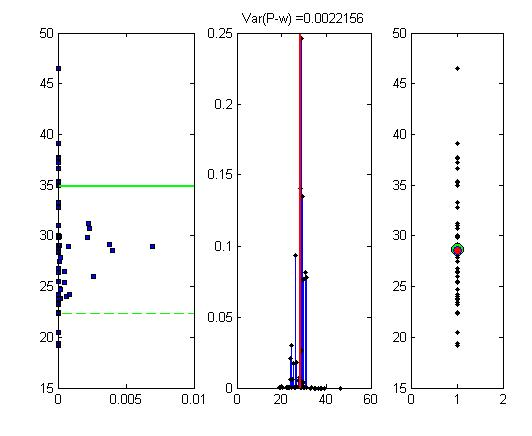
\includegraphics[scale=0.45]{Figures/Timestep16}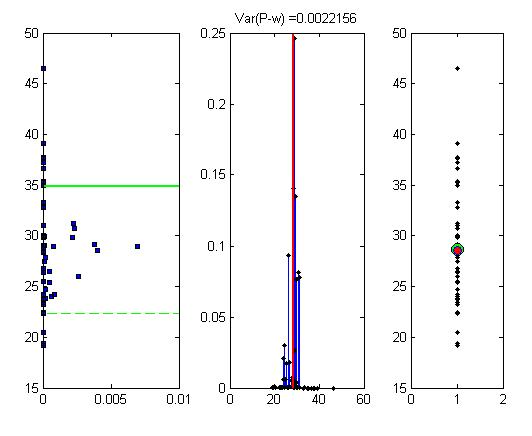
\includegraphics[scale=0.45]{Figures/Timestep43}
\par\end{centering}
}

\subfloat[$\left(t=71\right)$ et $\left(t=108\right)$]{\begin{centering}
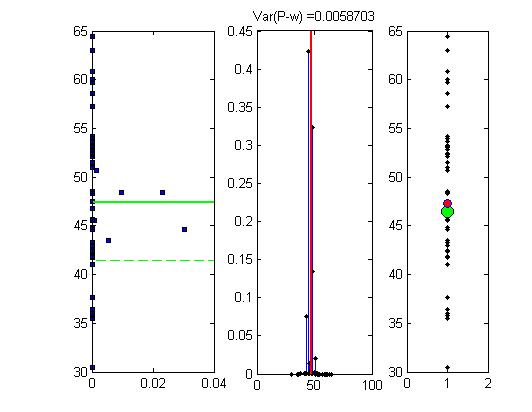
\includegraphics[scale=0.47]{Figures/Timestep71}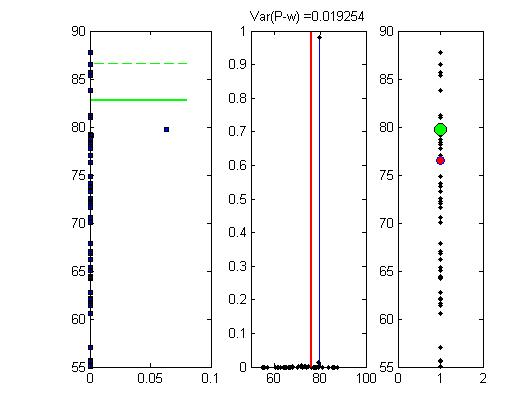
\includegraphics[scale=0.47]{Figures/Timestep108}
\par\end{centering}
}\caption{\label{fig:Probl=0000E8me-de-d=0000E9g=0000E9n=0000E9rescence}Probl�me
de d�g�n�rescence de poids}
\end{figure}

On constate que la variance des poids d'importances\textit{ }tend
� augmenter apr�s chaque it�ration, la d�g�n�rescence de poids est
in�vitable et cause une mauvais approximation de la loi a posteriori\textit{
}et donc une estimation fragile du niveau de d�gradation\textit{.
}De plus, ce probl�me implique que la plupart des ressources du centre
de calcul est affect� � propager les particules peu int�ressantes.

\begin{figure}
\begin{centering}
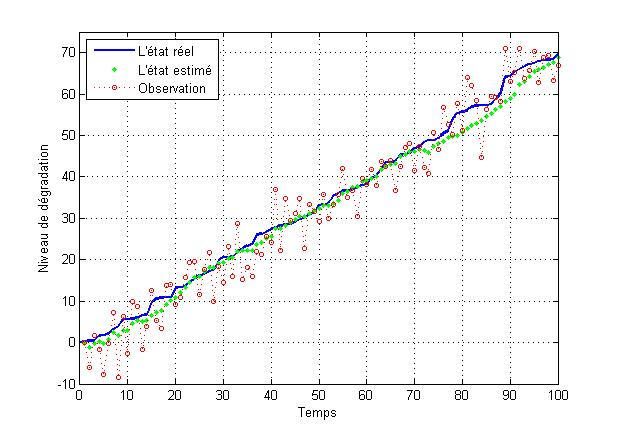
\includegraphics[scale=0.7]{Figures/Trajectoire}
\par\end{centering}
\caption{\label{fig:Trajectoire de l'=0000E9tat estim=0000E9}Trajectoire de
l'�tat estim�}
\end{figure}

La figure \textcolor{red}{\ref{fig:Trajectoire de l'=0000E9tat estim=0000E9}}
montre la trajectoire de l'�tat estim� obtenu apr�s 100 premi�res
it�rations. Les valeurs caract�risant l'�volution de 6 premi�res particules
sont enregistr�es dans le tableau \textcolor{red}{\ref{tab:=0000C9volutions des particules}}.

\begin{table}
\subfloat[Position des �chantillons]{\begin{centering}
\begin{tabular}{|c|c|c|c|c|c|c|c|}
\hline 
\multirow{2}{*}{$i$} & $\left(t=0\right)$ & \multicolumn{2}{c|}{$\left(t=1\right)$} & \multicolumn{2}{c|}{$\left(t=2\right)$} & \multicolumn{2}{c|}{$\left(t=3\right)$}\tabularnewline
\cline{2-8} \cline{3-8} \cline{4-8} \cline{5-8} \cline{6-8} \cline{7-8} \cline{8-8} 
 & $x_{\text{�}}P{}_{0}^{i}\equiv x_{-}P_{1}^{i}$ & $x_{-}P_{-}update{}_{1}^{i}$ & $x_{\text{�}}P{}_{2}^{i}$ & $x_{-}P_{-}update{}_{2}^{i}$ & $x_{\text{�}}P{}_{3}^{i}$ & $x_{-}P_{-}update{}_{3}^{i}$ & $\ldots$\tabularnewline
\hline 
1 & -0.5785 & \textcolor{blue}{-0.4927} & \textcolor{blue}{-0.4927} & \textcolor{red}{0.6983} & \textcolor{red}{0.6983} & 1.4469 & $\ldots$\tabularnewline
\hline 
2 & -0.7938 & \textcolor{blue}{1.1958} & \textcolor{blue}{1.1958} & \textcolor{red}{1.2958} & \textcolor{red}{1.2958} & 1.8700 & $\ldots$\tabularnewline
\hline 
3 & -1.2378 & \textcolor{blue}{-1.2223} & \textcolor{blue}{-1.2223} & \textcolor{red}{-0.6981} & \textcolor{red}{-0.6981} & -0.4150 & $\ldots$\tabularnewline
\hline 
4 & 9.0948 & \textcolor{blue}{9.3925} & \textcolor{blue}{9.3925} & \textcolor{red}{9.6794} & \textcolor{red}{9.6794} & 9.8049 & $\ldots$\tabularnewline
\hline 
5 & -6.7253 & \textcolor{blue}{-6.5783} & \textcolor{blue}{-6.5783} & \textcolor{red}{-5.9894} & \textcolor{red}{-5.9894} & -5.5064 & $\ldots$\tabularnewline
\hline 
6 & 0.9647 & \textcolor{blue}{1.2471} & \textcolor{blue}{1.2471} & \textcolor{red}{1.6316} & \textcolor{red}{1.6316} & 1.9371 & $\ldots$\tabularnewline
\hline 
$\ldots$ & $\ldots$ & $\ldots$ & $\ldots$ & $\ldots$ & $\ldots$ & $\ldots$ & $\ldots$\tabularnewline
\hline 
\end{tabular}
\par\end{centering}
}

\subfloat[Poids associ�s � chaque �chantillon]{\begin{centering}
\begin{tabular}{|c|c|c|c|c|c|c|c|c|c|c|}
\hline 
$i$ & $\left(t=0\right)$ & $\left(t=1\right)$ & $\left(t=2\right)$ & $\ldots$ & $\left(t=77\right)$ & $\left(t=78\right)$ & $\ldots$ & $\left(t=155\right)$ & $\left(t=156\right)$ & $\ldots$\tabularnewline
\hline 
1 & 0.02 & 0.024931 & 0.021084 & $\ldots$ & \textcolor{red}{0.027794} & \textcolor{red}{0.025749} & $\ldots$ & 2.26E-10 & 2.07E-10 & $\ldots$\tabularnewline
\hline 
2 & 0.02 & 0.024488 & 0.017501 & $\ldots$ & 9.56E-40 & 6.78E-40 & $\ldots$ & 3.06E-40 & 3.09E-40 & $\ldots$\tabularnewline
\hline 
3 & 0.02 & 0.024253 & 0.028749 & $\ldots$ & 1.19E-07 & 1.42E-07 & $\ldots$ & 1.75E-09 & 1.47E-09 & $\ldots$\tabularnewline
\hline 
4 & 0.02 & 0.004440 & 6.64E-05 & $\ldots$ & 3.47E-44 & 3.97E-44 & $\ldots$ & 3.60E-71 & 1.13E-71 & $\ldots$\tabularnewline
\hline 
5 & 0.02 & 0.010324 & 0.021677 & $\ldots$ & \textcolor{red}{0.007096} & \textcolor{red}{0.007282} & $\ldots$ & 2.71E-63 & 6.20E-64 & $\ldots$\tabularnewline
\hline 
6 & 0.02 & 0.024431 & 0.015785 & $\ldots$ & 0.000803 & 0.000994 & $\ldots$ & \textcolor{red}{0.998909} & \textcolor{red}{0.999447} & $\ldots$\tabularnewline
\hline 
$\ldots$ & $\ldots$ & $\ldots$ & $\ldots$ & $\ldots$ & $\ldots$ & $\ldots$ & $\ldots$ & $\ldots$ & $\ldots$ & $\ldots$\tabularnewline
\hline 
\end{tabular}
\par\end{centering}
}

\caption{\label{tab:=0000C9volutions des particules}�volutions de 6 premi�res
particules}
\end{table}

Au d�but, tous les �chantillons $\left\{ x_{0}^{i}\right\} _{i=1}^{N_{s}}$
sont assign�s un m�me valeur de poids d'importance $\omega_{0}^{i}=\frac{1}{N_{s}}$.
Quand le filtre d�marre, les particules sont propag�s ind�pendamment.
Apr�s 155 it�rations, on constate qu'il ne reste qu'un seul �chantillon
qui prend le poids approximativement � 1, alors que les poids des
autres �chantillons sont n�gligeables. On note aussi que un �chantillon
peut prendre le r�le le plus ``important'' durant quelques it�rations
avant de d�g�n�rer. 

\section{Distribution des �tats estim�s}

Dans cette section, on �tudie l'effet du SIS filtre particulaire sur
deux processus Gamma de l'incr�ment diff�rents:$\Gamma\left(k_{1},\theta_{1}\right)$
avec $\left(k_{1}=1;\theta_{1}=\frac{2}{3}\right)$ et $\Gamma\left(k_{2},\theta_{2}\right)$
avec $\left(k_{2}=\frac{1}{9},\theta_{2}=6\right)$. On peut observer
la densit� de probabilit� de ces deux distributions Gamma dans la
figure \textcolor{red}{\ref{fig:Densit=0000E9-de-probabilit=0000E9}}:

\begin{figure}
\subfloat[$\Gamma\left(k1,\theta1\right)$ avec $\left(k_{1}=1;\theta_{1}=\frac{2}{3}\right)$ ]{\begin{centering}
\includegraphics[scale=0.6]{Figures/a=1,b=1\lyxdot 5}
\par\end{centering}
}\subfloat[$\Gamma\left(k_{2},\theta_{2}\right)$ avec $\left(k_{2}=\frac{1}{9},\theta_{2}=6\right)$]{\begin{centering}
\includegraphics[scale=0.6]{\string"Figures/a = 1s9, b =1s6\string".eps}
\par\end{centering}
}\caption{\label{fig:Densit=0000E9-de-probabilit=0000E9}Densit� de probabilit�
de la distribution Gamma}
\end{figure}

Ces deux distributions Gamma ont le m�me moyenne alors que la variance
de $\Gamma\left(k_{2},\theta_{2}\right)$ est 9 fois plus grande que
celle de $\Gamma\left(k_{1},\theta_{1}\right)$:
\[
\begin{cases}
moyenne & =k_{1}\times\theta_{1}=k_{2}\times\theta_{2}=\frac{2}{3}\\
variance1 & =k_{1}\times\theta_{1}{}^{2}=1\times\left(\frac{2}{3}\right)^{2}=\frac{4}{9}\\
variance2 & =k_{2}\times\theta_{2}{}^{2}=\frac{1}{9}\times\left(6\right)^{2}=4
\end{cases}
\]

La figure \textcolor{red}{\ref{fig:Erreur-de-l'estimation}} montre
l'erreur de l'estimation $\left(d_{t}=\left(x_{MMSE}\right)_{t}-x_{t}\right)$
� chaque l'instant $\left(t\right)$ dans les deux cas $\Gamma\left(k_{1},\theta_{1}\right)$
et $\Gamma\left(k_{2},\theta_{2}\right)$ avec un bruit Gaussien de
moyenne nulle, l'�cart-type $\sigma_{\varepsilon}=5$. On trouve que
avec une m�me valeur de la variance $\left(\sigma_{\varepsilon}^{2}\right)$
du bruit de mesure, si l'incr�ment du processus Gamma est plus incertain,
la performance du filtre particulaire SIS d�cro�t fortement. La raison
est que quand on a un plus grand degr� de variabilit� sur la trajectoire
de l'�tat de d�gradation r�el $\left(x_{t}\right)$, les valeurs $\left\{ x_{-}P_{-}update_{t}^{i}\right\} _{i=1}^{N_{s}}$
et donc, $\left\{ y_{-}update_{t}^{i}\right\} _{i=1}^{N_{s}}$ se
dispersent davantage. Par cons�quent, les poids d'importances\textit{
}associ�s � ces �chantillons sont gravement �cart�s. Cela conduit
� une acc�l�ration du probl�me de d�g�n�rescence de poids.

\begin{figure}
\begin{centering}
\includegraphics[scale=0.7]{\string"Figures/Estimation Error\string".eps}
\par\end{centering}
\caption{\label{fig:Erreur-de-l'estimation}Erreur de l'estimation}
\end{figure}

Pour visualiser la vitesse de d�g�n�rescence de poids, on utilise
l'estimateur Maximum a Posteriori $\left(x_{MAP}\right)$:
\[
\left(x_{MAP}\right)_{t}=x_{t}^{i}\mid\text{W}_{t}^{i}=max\left\{ \text{W}_{t}^{i}\right\} _{i=1}^{N_{s}}
\]
Cet estimateur d�signe � chaque instant $\left(t\right)$ l'�chantillon
$\left(x_{t}^{i}\right)$ ayant le poids le plus fort, autrement dit
l'�chantillon le plus ``important'' au sens de la contribution �
l'estimation de l'�tat r�el. Lorsqu'il ne reste qu'un seul �chantillon
int�ressant, $\left(x_{MAP}\right)$ et $\left(x_{MMSE}\right)$ est
presque identique. La figure \textcolor{red}{\ref{fig:Vitesse-de-d=0000E9g=0000E9n=0000E9rescence}}
illustre cette id�e.

\begin{center}
\begin{figure}
\begin{centering}
\includegraphics[scale=0.4]{\string"Figures/Vitesse de d�g�n�rescence\string".eps}
\par\end{centering}
\caption{\label{fig:Vitesse-de-d=0000E9g=0000E9n=0000E9rescence}Vitesse de
d�g�n�rescence de poids }
\end{figure}
\par\end{center}

On peut trouver clairement que dans le cas d'un processus Gamma avec
la variance de l'incr�ment plus �lev�e, les poids d�g�n�rent plus
rapide. Cela diminue consid�rablement la qualit� du filtre particulaire
SIS.

Chaque fois on fait la simulation avec la m�me donn�e de mesure, on
obtient une trajectoire de l'�tat estim� tout � fait diff�rente. Donc,
pour �tudier la distribution des �tats estim�s � tous les instants,
on r�p�te par exemple 300 fois la proc�dure de filtrage. La figure
\textcolor{red}{\ref{fig:Distribution-des-=0000E9tats}} montrent
la distribution des �tats estim�s correspondante � certains instants
donn�s pour les deux incr�ments.

\begin{figure}
\begin{centering}
\subfloat[$\Gamma\left(k_{1},\theta_{1}\right)$ avec $\left(k_{1}=1,\theta_{1}=\frac{2}{3}\right)$]{\begin{centering}
\includegraphics[scale=0.4]{\string"Figures/Distribution � chaque instant (a)\string".eps}
\par\end{centering}
}
\par\end{centering}
\begin{centering}
\subfloat[$\Gamma\left(k_{2},\theta_{2}\right)$ avec $\left(k_{2}=\frac{1}{9},\theta_{2}=6\right)$]{\begin{centering}
\includegraphics[scale=0.4]{\string"Figures/Distribution � chaque instant (b)\string".eps}
\par\end{centering}
}
\par\end{centering}
\caption{\label{fig:Distribution-des-=0000E9tats}Distribution des �tats estim�s}
\end{figure}

\selectlanguage{french}

\selectlanguage{english}%

\chapter{Filtre particulaire SISR et l'estimation de la RUL}

Dans le quatri�me chapitre, on pr�sente d'abord le filtre particulaire
SISR (\textit{Sequential Importance Sampling and Resampling} en anglais)
developp� basant sur le SIS filtre particulaire. Ensuite, on parle
de l'estimation de la RUL et puis on analyse des r�sultats de simulation
et donne des remarques importantes. La loi du temps d'atteinte est
aussi abord�e dans ce chapitre.

\section{Filtre Bootstrap}

Comme on a vu dans le chapitre 3, un grave d�faut du filtre particulaire
SIS est le d�g�n�rescence de poids\textit{ }qui m�ne � une repr�sentation
inad�quate de la loi a posteriori\textit{. }Alors, il est indispensable
de penser � une technique qui vise � r�-initialiser le filtre r�guli�rement
pour pr�venir ce ph�nom�ne. L'id�e est d'introduire apr�s l'estimation
de l'�tat $\left(x_{t}\right)$, une �tape suppl�mentaire dite \textit{r�-�chantillonnage}
(ou \textit{redistribution}). Dans cette �tape, les �chantillons ayant
un poids faible sont �limin�s tandis que ceux dont le poids est fort
sont dupliqu�s et donc auront plus de chance d'approcher la loi a
posteriori � l'instant suivant. En g�n�ral, la redistribution\textit{
}peut �tre consid�r�e comme une autre �tape d'�chantillonnage d'importance\textit{
}dans laquelle la distribution discr�te pond�r�e $\left\{ x_{t}^{i},\text{W}_{t}^{i}\right\} _{i=1}^{N_{s}}$
est approch�e par un ensemble des �chantillons non pond�r�s (appel�s
les descendants) $\left\{ x_{t}^{i*}\right\} _{i*=1}^{N_{s}}$. De
cette mani�re l'�cart entre les poids d'importances\textit{ }� chaque
instant $\left(t\right)$ est r�duit et les particules peuvent �tre
mieux profit�s. Un algorithme de SIS filtre particulaire avec la redistribution\textit{
}� chaque instants $\left(t\right)$ est\textit{ }introduit dans \textcolor{green}{\cite{gordon1993novel}}
sous le nom \textit{filtre bootstrap .} Cet algorithme que l'on d�crit
dans \textcolor{red}{\ref{alg:filtre-bootstrap}} prend aussi le noyau
de transition\textit{ }comme la\textit{ }loi d'importance\textit{.}

\begin{algorithm}
\begin{centering}
\noindent\begin{minipage}[t]{1\columnwidth}%
\begin{center}
� l'instant $\left(t=0\right)$\linebreak{}
\par\end{center}
\begin{center}
\textbf{Initialisation}: $x_{0}^{i}\sim p\left(x_{0}\right),\,i=1:N_{s}$
\par\end{center}
\begin{center}
----------------------------------------------------------------------
\par\end{center}
\begin{center}
� partir de l'instant \textit{$\left(t\geq1\right)$ }\linebreak{}
\par\end{center}
\begin{center}
\textbf{�chantillonnage d'importance $\left(i=1:N_{s}\right)$}
\par\end{center}
\begin{center}
$\begin{cases}
x_{t}^{i}\sim p(x_{t}^{i}\mid x_{t-1}^{i})\\
\omega_{t}^{i}=p\left(y_{t}\mid x_{t}^{i}\right)
\end{cases}$
\par\end{center}
\begin{center}
\textbf{Normaliser}
\par\end{center}
\begin{center}
$\text{W}_{t}^{i}=\frac{\omega_{t}^{i}}{\sum_{i=1}^{N_{s}}\omega_{t}^{i}},\,i=1:N_{s}$
\par\end{center}
\begin{center}
\textbf{Estimer le niveau de d�gradation}
\par\end{center}
\begin{center}
$x_{MMSE}={\displaystyle \sum_{i=1}^{N_{s}}\text{W}_{t}^{i}\times x_{t}^{i}}$
\par\end{center}
\begin{center}
\textbf{Redistribution }$\left(i=1:N_{s}\right)$
\par\end{center}
\begin{center}
$x_{t}^{i*}=redistribution(x_{t}^{i},\,\text{W}_{t}^{i})$
\par\end{center}
\begin{center}
$\left(x_{t}^{i}=x_{t}^{i*}\right)$
\par\end{center}%
\end{minipage}
\par\end{centering}
\caption{\label{alg:filtre-bootstrap}Filtre bootstrap}
\end{algorithm}

Note que apr�s l'�tape de redistribution � l'instant $\left(t-1\right)$
les �chantillons ont des poids uniformes, donc il n'est pas n�cessaire
de sauvegarder ces poids pour l'instant $\left(t\right)$. Alors,
la formule qui sert � pond�rer les �chantillons � l'instant $\left(t\right)$
est tr�s simple $\omega_{t}^{i}=p\left(y_{t}\mid x_{t}\right)$ (pas
de multiplication r�cursive). L'utilisation du\textit{ }noyau de transition
comme la loi d'importance est tr�s populaire car quand le probl�me
change (l'�quation d'�tat change), on ne doit que corriger l'expression
du noyau de transition et de la fonction de vraisemblance\textit{
}dans le programme\textit{. }

Selon \textcolor{green}{\cite{casella1996statistical}}, \textcolor{green}{\cite{carpenter1999improved}}
et \textcolor{green}{\cite{johansen2007monte}}, l'�tape de redistribution\textit{
}engendre extra Monte Carlo variance de l'estimateur. Donc, on est
recommand� d'effectuer pr�alablement l'estimation de l'�tat de d�gradation
� chaque instant � l'aide des �chantillons pond�r�s.

Le m�canisme de redistribution\textit{ }est illustr�e dans la figure
\textcolor{red}{\ref{fig:Proc=0000E9dure-de-r=0000E9distribution}}.

\begin{figure}
\begin{centering}
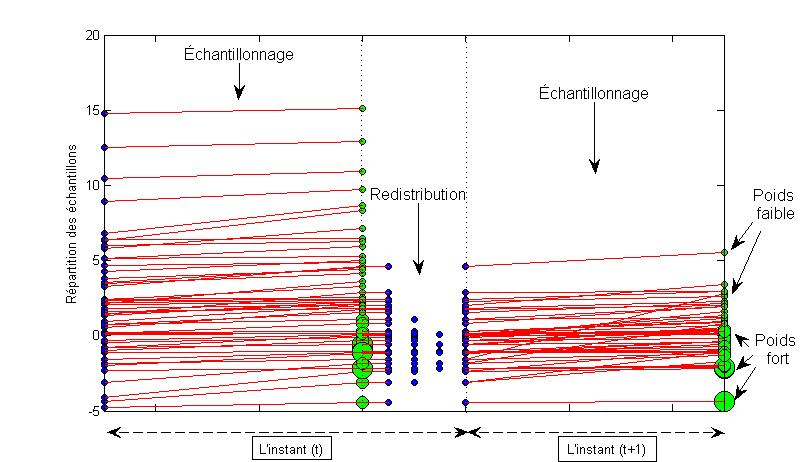
\includegraphics[scale=0.5]{Figures/Resampling}
\par\end{centering}
\caption{\label{fig:Proc=0000E9dure-de-r=0000E9distribution}M�canisme de redistribution}
\end{figure}

En g�n�ral, le filtre bootstrap\textit{ }ne donne plus une approximation
efficace de la loi a posteriori\textit{ }quand le temps T $\left(t=1:T\right)$
est tr�s grand � cause des redistributions successives. En effet,
le m�canisme de redistribution\textit{ }r�duit\textit{ }la diversit�
des particules, c'est-�-dire quand le temps passe, l'ensemble des
particules contient seulement quelques unes ``distingu�es''. La
plupart entre eux sont des descendants d'un m�me anc�tre. C'est �videmment
la cons�quence d'effectuer l'�chantillonnage d'une distribution discr�te
au lieu d'une distribution continue. Ce ph�nom�ne qu'on appelle \textit{d�g�n�rescence
des positions} (\textit{sample imporverishment} en anglais) a le m�me
effet que la d�g�n�rescence de poids\textit{ }mentionn�e dans le chapitre
3. D'apr�s \textcolor{green}{\cite{avitzour1995stochastic}}, si le
bruit du processus (l'incr�ment $\Gamma\left(k,\theta\right)$ du
processus Gamma) a une variance suffisamment grande, les �chantillons
non pond�r�s $\left\{ x_{t}^{i*}\right\} _{i=1}^{N_{s}}$ peuvent
�tre propag�s, dans l'�tape de pr�diction � l'instant suivant, de
sorte qu'ils peuvent maintenir une diversit� ad�quate au sein de l'ensemble
d'�chantillons. Au contraire, si $\left\{ x_{t}^{i*}\right\} _{i=1}^{N_{s}}$
ne sont pas suffisamment contrebalanc�s par le bruit du processus,
la qualit� de l'approximation de la loi a\textit{ }posteriori est
d�grad�e. Pour r�soudre ce probl�me, des mesures sont propos�es et
recapitul�es dans \textcolor{green}{\cite{gordon1993novel}}, \textcolor{green}{\cite{arulampalam2002tutorial}},
\textcolor{green}{\cite{gustafsson2002particle}}, \textcolor{green}{\cite{legland2003filtrage}}
et \textcolor{green}{\cite{doucet2009tutorial}}.

\section{Filtre SISR avec redistribution d'adaptation \label{sec:Variants}}

Pour obtenir une estimation du niveau de d�gradation plus exacte �
chaque instant $\left(t\right)$, il est possible de modifier l'\textcolor{red}{\ref{alg:filtre-bootstrap}}
sur les points suivants:
\begin{labeling}{00.00.0000}
\item [{-}] La redistribution multinomiale est la plus simple technique
par l'utilisation delaquelle $N_{s}$ nouveaux �chantillons (les descendants)
sont s�lectionn�es � partir de $N_{s}$ ancients �chantillons avec
la probabilit� �gale � leurs poids normalis�s: $p\left(x_{t}^{i*}=x{}_{t}^{i}\right)=\text{W}_{t}^{i}$.
En choissisant d'autres techniques de redistribution on peut r�duire
la variance introduite par l'�tape de redistribution\textit{.} L'une
est la technique de redistribution syst�matique propos�e par Kitagawa
\textcolor{green}{\cite{kitagawa1996monte}} et l'autre est la redistribution
des r�sidus introduite par Liu et Chen \textcolor{green}{\cite{liu1998sequential}}.
Une comparaison sur la qualit� et la complexit� de ces trois techniques
est effectu� dans \textcolor{green}{\cite{douc2005comparison}} et
\textcolor{green}{\cite{hol2006resampling}}. Dans ce rapport les
r�sultats de la simulation sont obtenus avec l'utilisation de la technique
de redistribution de Kitagawa dont le code est donn� dans \textcolor{green}{\cite{campillo2006filtrage}}. 
\item [{-}] On peut am�liorer la performance du filtre particulaire en
augmentant le nombre d'�chantillons. N�anmoins, cela ne para�t pas
comme une solution pratique. Il est pr�f�rable de choisir une meilleure
loi d'importance\textit{.} \textcolor{green}{\cite{cappe2007overview}}
donne un bon r�sum� sur cette alternative . Une loi d'importance\textit{
}optimale obtenu dans un cas particulier est repr�sent� dans \textcolor{green}{\cite{doucet2000sequential}}
et \textcolor{green}{\cite{arulampalam2002tutorial}}.
\item [{-}] On sait maintenant que l'on ne doit pas redistribuer � chaque
instant mais de le faire de telle mani�re que la redistribution puisse
pr�venir la\textit{ }d�g�n�rescence de poids\textit{ }et ne cause
pas une d�g�n�rescence des positions\textit{ }trop grave. Autrement
dit, les �chantillons sont redistribu�s seulement quand un grand d�s�quilibre
de leurs poids d'importances est constat�. Alors, on souhaite de disposer
une crit�re qui nous permet de d�terminer s'il est n�cessaire de redistribuer
les �chantillons ou s'il faut les conserver. \textcolor{green}{\cite{kong1994sequential}},
\textcolor{green}{\cite{liu1995blind}} quantifient le niveau de d�s�quilibre
des poids d'importances en utilisant un coefficient appel� nombre
d'�chantillons effectives:
\[
N_{eff}\approx\frac{1}{\sum_{i=1}^{N_{s}}\left(\text{W}_{t}^{i}\right)^{2}}\in\left[1,N_{s}\right]
\]
\end{labeling}
Lorsque $N_{eff}$ est proche de $N_{s}$, les �chantillons contribuent
de fa�on �gale � l'approximation de la loi a posteriori\textit{ }tandis
que une valeur proche de 1 indique une d�g�n�rescence de poids\textit{
}s�v�re. La redistribution est faite seulement quand $N_{eff}$ est
inf�rieur � un seuil $N_{thresh}$ pr�d�termin�, typiquement $N_{thresh}=\frac{N_{s}}{2}$.

Tenir compte de la premier et de la troisi�me modification mentionn�es
au dessus, un algorithme du filtre SISR avec redistribution d'adaptation
est pr�sent� dans l'\textcolor{red}{\ref{alg:-Filtre-adaptive}}.

\begin{algorithm}
\begin{centering}
\noindent\begin{minipage}[t]{1\columnwidth}%
\begin{center}
� l'instant $\left(t=0\right)$\linebreak{}
\par\end{center}
\begin{center}
\textbf{Initialisation}:$\begin{cases}
x_{0}^{i} & \sim p\left(x_{0}\right)\\
\omega_{0}^{i} & =\nicefrac{1}{N_{s}}
\end{cases},\,i=1:N_{s}$
\par\end{center}
\begin{center}
-----------------------------------------------------------------------
\par\end{center}
\begin{center}
� partir de l'instant \textit{$\left(t\geq1\right)$}\linebreak{}
\par\end{center}
\begin{center}
\textbf{�chantillonnage d'importance}
\par\end{center}
\begin{center}
$\begin{cases}
x_{t}^{i} & \sim p(x_{t}^{i}\mid x_{t-1}^{i})\\
\omega_{t}^{i} & =\omega_{t}^{i}\times p\left(y_{t}\mid x_{t}^{i}\right)
\end{cases}$
\par\end{center}
\begin{center}
\textbf{Normaliser}
\par\end{center}
\begin{center}
$\text{W}_{t}^{i}=\frac{\omega_{t}^{i}}{\sum_{i=1}^{N_{s}}\omega_{t}^{i}},\,i=1:N_{s}$
\par\end{center}
\begin{center}
\textbf{Estimer le niveau de d�gradation}
\par\end{center}
\begin{center}
$x_{MMSE}={\displaystyle \sum_{i=1}^{N_{s}}\text{W}_{t}^{i}\times x_{t}^{i}}$
\par\end{center}
\begin{center}
\textbf{Calculer le nombre d'�chantillons effectives}
\par\end{center}
\begin{center}
$N_{eff}=\frac{1}{{\displaystyle \sum_{i=1}^{N_{s}}\left(\text{W}_{t}^{i}\right)^{2}}}$
\par\end{center}
\begin{center}
Si $N_{eff}\leq N_{thresh}$ alors
\par\end{center}
\begin{center}
\textbf{Redistribution }$\left(i=1:N_{s}\right)$
\par\end{center}
\begin{center}
$x_{t}^{i*}=redistribution(x_{t}^{i},\,\text{W}_{t}^{i})$
\par\end{center}
\begin{center}
$\begin{cases}
x_{t}^{i}=x{}_{t}^{i*}\\
\omega_{t}^{i}=\nicefrac{1}{N}_{s}
\end{cases}$
\par\end{center}%
\end{minipage}
\par\end{centering}
\caption{\label{alg:-Filtre-adaptive} Filtre SISR avec redistribution d'adaptation\textit{.}}
\end{algorithm}

Comme on a dit au dessus, la redistribution\textit{ }donne effectivement
des ``bruits'' additionnels. Cependant, redistribuer des �chantillons
nous aide � �viter l'accumulation des erreurs avec le temps et donc
rendre l'approximation de la loi a posteriori plus stable \textcolor{green}{\cite{doucet2009tutorial}}
, \textcolor{green}{\cite{cappe2007overview}}. C'est la raison pourlaquelle
la redistribution est largement utilis�e. En pratique, impl�menter
correctement l'�tape de redistribution peut am�liorer vivement la
performance du filtre particulaire. Pour illustrer cette id�e, on
d�fini tout d'abord un indicateur qui d�signe l'erreur quadratique
moyenne de l'estimation � chaque instant $\left(t\right)$:
\begin{equation}
RMSE_{t}=\sqrt{\frac{1}{300}\times\sum_{k=1}^{300}\left(\left(x_{MMSE}\right)_{t}^{k}-x_{t}\right)^{2}}\label{eq:RMSE_t}
\end{equation}
avec l'ensemble$\left\{ \left(x_{MMSE}\right)_{t}^{k}\right\} _{k=1}^{300}$
contient 300 valeurs estim�es du niveau de d�gradation r�el $\left(x_{t}\right)$
� chaque instant $\left(t=1:500\right)$, obtenues apr�s k = 300 it�rations.

En utilisant les algorithmes \textcolor{red}{\ref{alg:Algorithme SIS filtre particulaire}}
et \textcolor{red}{\ref{alg:-Filtre-adaptive}}, on obtient pour chacun
les valeurs $RMSE_{t}$ ainsi que les variance $var\left(\left\{ \left(x_{MMSE}\right)_{t}^{k}\right\} _{k=1}^{300}\right)$
� chaque instant $\left(t=1:500\right)$ correspondantes. Les avantages
de l'utilisation d'un filtre SISR avec redistribution d'adaption au
lieu d'un SIS filtre particulaire est indiquer dans la figure \textcolor{red}{\ref{fig:RMSE_t}}.

\begin{figure}
\subfloat[SIS filtre particulaire]{\includegraphics[scale=0.3]{\string"Figures/RMSE � chaque instant (a)\string".eps}

\includegraphics[scale=0.3]{\string"Figures/variance � chaque instant (a)\string".eps}

}

\subfloat[Filtre SISR avec redistribution adaptive]{\includegraphics[scale=0.3]{\string"Figures/RMSE � chaque instant (b)\string".eps}

\includegraphics[scale=0.3]{\string"Figures/variance � chaque instant (b)\string".eps}

}

\caption{\label{fig:RMSE_t}$RMSE_{t}$ et $var\left(\left\{ \left(x_{MMSE}\right)_{t}^{k}\right\} _{k=1}^{300}\right)$
� chaque instant $\left(t=1:500\right)$ }
\end{figure}

La trajectoire de $RMSE_{t}$ dans la figure \textcolor{red}{\ref{fig:RMSE_t}}
n'est pas monotone, ce qui nous mette en difficult� � donner une conclusion
certaine sur l'exactitude de l'estimation du niveau de d�gradation.
Plus pr�cis�ment, il est probable qu'un grand nombre de mesures effectu�es
n'assurent pas une am�lioration de la qualit� de l'estimation. En
effet, l'utilisation beaucoup de donn�es bruit�es peuvent diminuer
la performance du filtre particulaire. Alors, on pense � utiliser
de mani�re plus intelligemment un moindre donn�es pour les profiter
mais sans avoir perturber le filtre particulaire.

\section{Estimation de la RUL}

Rappelons que l'instant courant est $\left(t_{n}=500\right)$. Pour
calculer la vie r�siduelle, on propage le processus Gamma avec le
niveau de d�gradation initial $\left(x_{MMSE}\right)_{t=500}^{k},k=1:300$
jusqu'au moment $\left(t\right)$ o� $\left(x_{MMSE}\right)_{t}^{k}$
atteint un seuil pr�d�termin� appel� seuil de d�faillance. Alors,
si la date de d�faillance pr�vue est not�e $T_{d\acute{e}f}$, la
RUL correspondant est:
\[
RUL=T_{d\acute{e}f}-t_{n}=T_{d\acute{e}f}-500
\]
En r�p�tant cette proc�dure $k=300$ fois, on obtient la distribution
de la RUL.

Avant de faire la simulation, il est indispensable de d�terminer le
seuil de d�faillance $S_{d\acute{e}f}$. Suppose que la date de d�faillance
r�el est $T_{d\acute{e}f}=600$, donc la RUL r�elle est 100. La figure
\textcolor{red}{\ref{fig:Seuil-de-d=0000E9faillance}} montre que
le seuil de d�faillance correspondant de deux processus Gamma de l'incr�ment
$\Gamma\left(k_{1}=1,\theta_{1}=\nicefrac{2}{3}\right)$ et $\Gamma\left(k_{2}=\nicefrac{1}{9},\theta_{2}=6\right)$
est 424.5 et 347.4 respectivement.

\begin{center}
\begin{figure}[h]
\begin{centering}
\includegraphics[scale=0.7]{\string"Figures/Seui de d�faillance\string".eps}
\par\end{centering}
\caption{\label{fig:Seuil-de-d=0000E9faillance}Seuil de d�faillance}
\end{figure}
\par\end{center}

L'�volution du niveau de d�gradation est montr�e dans la figure \textcolor{red}{\ref{fig:Estimation-de-la}}.
La distribution de la RUL estim�e est dessin�e en couleur verte.

\begin{figure}[h]
\begin{centering}
\subfloat[Processus Gamma de l'incr�ment $\Gamma\left(k_{1}=1,\theta_{1}=\nicefrac{2}{3}\right)$]{\begin{centering}
\includegraphics[scale=0.25]{\string"Figures/Estimation de la RUL (a)\string".eps}
\par\end{centering}
\begin{centering}
\includegraphics[scale=0.25]{\string"Figures/Estimation de la RUL en fonction de temps (a)\string".eps}
\par\end{centering}
}
\par\end{centering}
\begin{centering}
\subfloat[Processus Gamma de l'incr�ment $\Gamma\left(k_{2}=\nicefrac{1}{9},\theta_{2}=6\right)$]{\begin{centering}
\includegraphics[scale=0.25]{\string"Figures/Estimation de la RUL (b)\string".eps}
\par\end{centering}
\begin{centering}
\includegraphics[scale=0.25]{\string"Figures/Estimation de la RUL en fonction de temps (b)\string".eps}
\par\end{centering}
}
\par\end{centering}
\caption{\label{fig:Estimation-de-la}Estimation de la RUL}
\end{figure}


\section{R�sultats de simulation}

Dans cette section, on cherche � comprendre l'impact de deux param�tres:
nombre d'�chantillons $\left(N_{s}\right)$ et l'�cart-type du bruit
de mesures $\left(\sigma_{\varepsilon}\right)$ sur la performance
du filtre particulaire.

\subsection{Quand le nombre d'�chantillons $\left(N_{s}\right)$ augmente}

D'abord, on introduit un nouveau indicateur $RMSE_{globale}$ pour
avoir une vue globale sur l'importance des param�tres comme le nombre
d'�chantillons $N_{s}$ et l'�cart-type du bruit de mesures $\sigma_{\varepsilon}$:
\[
RMSE_{globale}^{k}=\sqrt{\frac{1}{T}\sum_{t=1}^{T}\left(\left(x_{MMSE}\right)_{t}^{k}-x_{t}\right)^{2}}
\]
Car � chaque simulation $\left(k\right)$, le filtre particulaire
produit une diff�rente trajectoire du niveau de d�gradation estim�
$\left\{ x_{MMSE}\right\} _{t=1}^{T},T=500$, donc les valeurs $RMSE_{globale}$
affich�es dans les tableaux suivants est la moyenne des valeurs $RMSE_{globale}^{k}$
obtenues apr�s $\left(k=300\right)$ simulations. Plus on obtient
un $RMSE_{globale}$ petit, plus il est probable que l'on peut avoir
une estimation pr�cise.

Calcul�e selon la formule \textcolor{blue}{\eqref{eq:RMSE_t}} avec
$\left(t=500\right)$, $RMSE_{t_{n}=500}$ d�signe l'erreur de l'estimation
du niveau de d�gradation � l'instant courant.

Un troisi�me indicateur utilis� est $RMSE_{RUL}$ qui indique l'erreur
de l'estimation de la RUL par rapport � la RUL r�elle (=100):
\[
RMSE_{RUL}=\sqrt{\frac{1}{300}\times\sum_{k=1}^{300}\left(\left(RUL\right)_{k}-100\right)^{2}}
\]

Les r�sultats de simulation sont pr�sent�s dans les tableaux suivantes:

\begin{center}
\begin{tabular}{|c|c|c|c|c|c|c|}
\hline 
\multirow{3}{*}{$N_{s}$} & \multicolumn{6}{c|}{$\Gamma\left(k_{1}=1,\theta_{1}=\nicefrac{2}{3}\right),\sigma_{\varepsilon}=5$}\tabularnewline
\cline{2-7} \cline{3-7} \cline{4-7} \cline{5-7} \cline{6-7} \cline{7-7} 
 & \multicolumn{3}{c|}{SIS filtre particulaire} & \multicolumn{3}{c|}{Filtre SISR avec redistribution d'adaptation}\tabularnewline
\cline{2-7} \cline{3-7} \cline{4-7} \cline{5-7} \cline{6-7} \cline{7-7} 
 & $RMSE_{globale}$ & $RMSE_{t_{n}=500}$ & $RMSE_{RUL}$ & $RMSE_{globale}$ & $RMSE_{t_{n}=500}$ & $RMSE_{RUL}$\tabularnewline
\hline 
50 & 4.832 & 7.963 & 37.771 & 2.074 & 3.705 & 34.473\tabularnewline
\hline 
100 & 4.390 & 8.114 & 36.933 & 2.047 & 3.643 & 34.430\tabularnewline
\hline 
300 & 4.030 & 6.798 & 35.375 & 2.033 & 3.494 & 35.741\tabularnewline
\hline 
500 & 3.890 & 7.604 & 38.099 & 2.031 & 3.490 & 35.005\tabularnewline
\hline 
1000 & 3.671 & 7.394 & 37.463 & 2.027 & 3.448 & 33.568\tabularnewline
\hline 
2000 & 3.539 & 7.232 & 36.946 & 2.028 & 3.473 & 35.628\tabularnewline
\hline 
4000 & 3.354 & 7.357 & 36.725 & 2.025 & 3.444 & 33.866\tabularnewline
\hline 
7000 & 3.240 & 7.140 & 36.827 & 2.025 & 3.440 & 34.400\tabularnewline
\hline 
10000 & 3.179 & 6.623 & 35.948 & 2.025 & 3.429 & 33.925\tabularnewline
\hline 
\end{tabular}
\par\end{center}

\begin{center}
\begin{tabular}{|c|c|c|c|c|c|c|}
\hline 
\multirow{3}{*}{$N_{s}$} & \multicolumn{6}{c|}{$\Gamma\left(k_{2}=\nicefrac{1}{9},\theta_{2}=6\right),\sigma_{\varepsilon}=5$}\tabularnewline
\cline{2-7} \cline{3-7} \cline{4-7} \cline{5-7} \cline{6-7} \cline{7-7} 
 & \multicolumn{3}{c|}{SIS filtre particulaire} & \multicolumn{3}{c|}{Filtre SISR avec redistribution d'adaptation}\tabularnewline
\cline{2-7} \cline{3-7} \cline{4-7} \cline{5-7} \cline{6-7} \cline{7-7} 
 & $RMSE_{globale}$ & $RMSE_{t_{n}=500}$ & $RMSE_{RUL}$ & $RMSE_{globale}$ & $RMSE_{t_{n}=500}$ & $RMSE_{RUL}$\tabularnewline
\hline 
50 & 11.237 & 19.822 & 44.955 & 2.498 & 4.608 & 41.677\tabularnewline
\hline 
100 & 9.980 & 14.886 & 44.364 & 2.392 & 4.144 & 40.025\tabularnewline
\hline 
300 & 8.801 & 11.447 & 42.990 & 2.311 & 4.117 & 40.475\tabularnewline
\hline 
500 & 8.361 & 11.570 & 42.283 & 2.298 & 4.116 & 42.015\tabularnewline
\hline 
1000 & 7.955 & 10.604 & 43.700 & 2.282 & 4.086 & 41.021\tabularnewline
\hline 
2000 & 7.467 & 10.499 & 39.610 & 2.278 & 4.117 & 38.559\tabularnewline
\hline 
4000 & 7.171 & 9.137 & 45.841 & 2.275 & 4.136 & 42.825\tabularnewline
\hline 
7000 & 6.846 & 9.406 & 43.610 & 2.274 & 4.126 & 40.738\tabularnewline
\hline 
10000 & 6.680 & 8.471 & 42.690 & 2.274 & 4.127 & 38.779\tabularnewline
\hline 
\end{tabular}
\par\end{center}

Avec le SIS filtre particulaire, on trouve que plus $\left(N_{s}\right)$
est grand, plus $RMSE_{globale}$ d�croit. N�anmoins, pour la raison
sp�cifi�e dans la section \textcolor{red}{\ref{sec:Variants}}, une
valeur $RMSE_{globale}$ petite n'assure pas une erreur de l'estimation
petite. Par ailleurs, avec un grand $\left(N_{s}\right)$, le filtre
particulaire donne des valeurs $RMSE_{globale}$ et $RMSE_{t_{n}=500}$
plus robuste.

En utilisant un SIS filtre particulaire, le processus Gamma dont l'incr�ment
$\Gamma\left(k_{2}=\nicefrac{1}{9},\theta_{2}=6\right)$ ayant une
variance plus grande offre des erreurs $RMSE_{globale}$, $RMSE_{t_{n}=500}$
et dans une certaine mesure, $RMSE_{RUL}$ plus grandes. C'est parce
que un tel processus subit une d�g�n�rescence de poids plus s�v�re.
Avec l'algorithme du filtre SISR avec redistribution d'adaptation,
la diff�rence entre les deux processus Gamma au vu des indicateurs
$RMSE_{globale}$ et $RMSE_{t_{n}=500}$ est r�duite. Pourtant, $RMSE_{RUL}$
reste encore diff�r� significativement car l'estimation de la RUL
est fortement influenc� par la variance de l'incr�ment (voir figure
\textcolor{red}{\ref{fig:Estimation-de-la}}). C'est aussi la raison
pourlaquelle un bon diagnostic n'assure pas un bon r�sultat de prognostic,
notamment dans le cas du processus Gamma avec un incr�ment tr�s vari�
$\left(\Gamma\left(k_{2}=\nicefrac{1}{9},\theta_{2}=6\right)\right)$. 

Par rapport au SIS filtre particulaire, l'impl�tation de l'�tape de
redistribution d'adaptation apporte une erreur $RMSE_{globale}$ beaucoup
plus petite. De plus, comme l'erreur de l'estimation du niveau de
d�gradation courante (le diagnostic) est plus petite, on obtient une
l�g�re am�lioration du r�sultat de prognostic. Enfin, on constate
que l'augmentation de $N_{s}$ n'apporte pas une am�lioration importante
pour les r�sultats $RMSE_{globale}$ et $RMSE_{t_{n}=500}$.

\subsection{Quand l'�cart-type du bruit de mesures $\left(\sigma_{\varepsilon}\right)$
varie}
\begin{center}
\begin{tabular}{|c|c|c|c|c|c|c|}
\hline 
\multirow{3}{*}{$\sigma_{\varepsilon}$} & \multicolumn{6}{c|}{Filtre SISR avec redistribution d'adaptation, $N_{s}=1000$}\tabularnewline
\cline{2-7} \cline{3-7} \cline{4-7} \cline{5-7} \cline{6-7} \cline{7-7} 
 & \multicolumn{3}{c|}{$\Gamma\left(k_{1}=1,\theta_{1}=\nicefrac{2}{3}\right)$} & \multicolumn{3}{c|}{$\Gamma\left(k_{2}=\nicefrac{1}{9},\theta_{2}=6\right)$}\tabularnewline
\cline{2-7} \cline{3-7} \cline{4-7} \cline{5-7} \cline{6-7} \cline{7-7} 
 & $RMSE_{globale}$ & $RMSE_{t_{n}=500}$ & $RMSE_{RUL}$ & $RMSE_{globale}$ & $RMSE_{t_{n}=500}$ & $RMSE_{RUL}$\tabularnewline
\hline 
3 & 1.315 & 0.731 & 32.448 & 1.651 & 0.088 & 42.868\tabularnewline
\hline 
4 & 1.672 & 1.096 & 32.862 & 2.222 & 1.089 & 42.196\tabularnewline
\hline 
5 & 2.027 & 3.448 & 33.568 & 2.282 & 4.086 & 41.021\tabularnewline
\hline 
6 & 1.838 & 1.622 & 33.164 & 2.474 & 2.778 & 39.873\tabularnewline
\hline 
7 & 2.130 & 2.543 & 33.274 & 3.047 & 0.139 & 42.628\tabularnewline
\hline 
8 & 2.052 & 3.207 & 33.810 & 3.353 & 5.528 & 38.409\tabularnewline
\hline 
9 & 2.444 & 5.939 & 36.720 & 3.268 & 2.024 & 40.908\tabularnewline
\hline 
10 & 2.479 & 2.305 & 33.661 & 3.840 & 0.395 & 40.508\tabularnewline
\hline 
11 & 2.371 & 4.618 & 35.367 & 3.862 & 5.658 & 44.118\tabularnewline
\hline 
12 & 2.512 & 6.597 & 37.228 & 3.873 & 2.052 & 42.148\tabularnewline
\hline 
13 & 3.546 & 4.706 & 36.088 & 3.839 & 0.720 & 43.288\tabularnewline
\hline 
14 & 2.526 & 4.077 & 35.697 & 4.562 & 3.367 & 42.462\tabularnewline
\hline 
15 & 3.489 & 7.957 & 38.998 & 5.043 & 0.923 & 39.909\tabularnewline
\hline 
16 & 3.354 & 10.794 & 41.591 & 5.645 & 6.238 & 39.731\tabularnewline
\hline 
17 & 3.445 & 2.592 & 32.583 & 4.482 & 0.628 & 40.944\tabularnewline
\hline 
\end{tabular}
\par\end{center}

Comme on a dit dans la section \textcolor{red}{\ref{sec:Loi-d'importance}},
choisir la loi d'importance sous la forme du noyau de transition emm�ne
� un filtre particuli�rement sensible avec des observations bruit�es.
Par cons�quent, la qualit� de l'estimation est instable (cette id�e
est illustr�e dans la figure \textcolor{red}{\ref{fig:Variation-RMSE-globale}}
o� les graphes $RMSE_{globale}$ sont non lin�aires, non monotones). 

D'autre part, on constate que m�me si $\sigma{}_{\varepsilon}$ est
grand, le filtre particuliare peut apporte un bon diagnostic si la
variance de la distribution $\Gamma\left(k,\theta\right)$ est suffisamment
petite . Alors que si cette variance est grande, le diagnostic est
arbitrairement de mauvaise qualit� m�me si $\sigma{}_{\varepsilon}$
est petit. Par exemple, avec l'incr�ment $\Gamma\left(k_{1}=1,\theta_{1}=\nicefrac{2}{3}\right)$,
$RMSE_{t_{n}=500}=4.077$ quand $\sigma{}_{\varepsilon}=14$ tandis
que $RMSE_{t_{n}=500}=4.086$ quand $\sigma{}_{\varepsilon}=8$ avec
l'incr�ment $\Gamma\left(k_{2}=\nicefrac{1}{9},\theta_{2}=6\right)$.

\begin{figure}
\begin{centering}
\subfloat[\label{fig:Variation-RMSE-globale}Variation de $RMSE_{globale}$
lorsque $\left(\sigma{}_{\varepsilon}\right)$ change ]{\begin{centering}
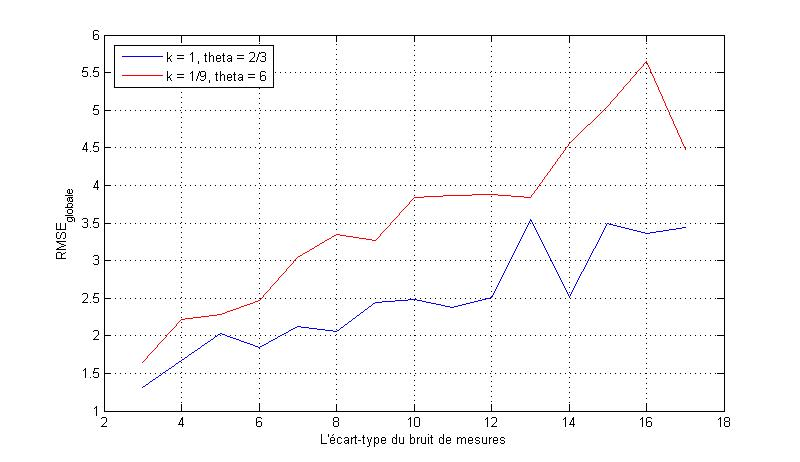
\includegraphics[scale=0.5]{Figures/F17}
\par\end{centering}
}
\par\end{centering}
\begin{centering}
\subfloat[Variation de $RMSE_{t_{n}=500}$ et $RMSE_{RUL}$ lorsque $\left(\sigma{}_{\varepsilon}\right)$
change]{\begin{centering}
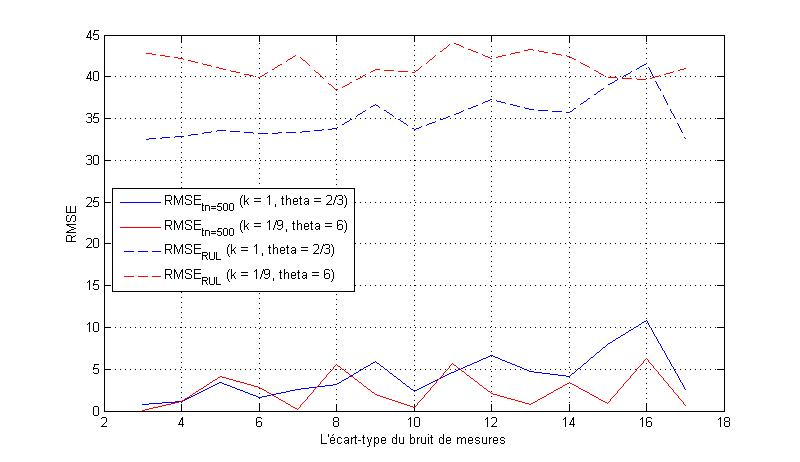
\includegraphics[scale=0.5]{Figures/F16}
\par\end{centering}
}
\par\end{centering}
\caption{Impact de l'�cart-type du bruit de mesures $\left(\sigma_{\varepsilon}\right)$}
\end{figure}


\subsection{Loi du temps d'atteinte}

Le temps d'atteinte (\textit{first hitting time} - FHT en anglais)
est l'instant o� le niveau de d�gradation d�passe le seuil de d�faillance.
La densit� de probabilit� de FHT en fonction du temps est montr�e
dans la figure \textcolor{red}{\ref{fig:Densit=0000E9-de-la}}. On
trouve que cette densit� de probabilit� devient plus �troite quand
l'instant courant approche la date de d�faillance $T_{d\acute{e}f}=600$.
Cela signifie que l'estimation de FHT est plus exacte quand le temps
passe.

\begin{figure}[h]
\begin{centering}
\subfloat[Incr�ment $\Gamma\left(k_{1}=1,\theta_{1}=\nicefrac{2}{3}\right)$]{\begin{centering}
\includegraphics[scale=0.4]{\string"Figures/Loi du temps d'atteinte (a)\string".eps}
\par\end{centering}
}
\par\end{centering}
\begin{centering}
\subfloat[Incr�ment $\Gamma\left(k_{2}=\nicefrac{1}{9},\theta_{2}=6\right)$]{\begin{centering}
\includegraphics[scale=0.4]{\string"Figures/Loi du temps d'atteinte (b)\string".eps}
\par\end{centering}
}
\par\end{centering}
\caption{\label{fig:Densit=0000E9-de-la}Densit� de probabilit� de la loi du
temps d'atteinte}
\end{figure}




\chapter{Conclusion}

L'objectif de ce stage durant six mois est d'�tudier une approche
stochastique dite filtre particulaire pour r�soudre le probl�me de
diagnostic et prognostic de d�faillance. Le processus Gamma est choisi
pour mod�liser la d�gradation. Apr�s avoir chercher � comprendre comment
un filtre particulaire est construit, on mette en application des
algorithmes fondamentales afin de r�aliser l'estimation du niveau
de d�gradation actuel et puis calculer la dur�e de vie r�siduelle
du syst�me d'int�r�t. Dans la simulation, on �tudie la performance
du filtre particulaire lors d'une variation des param�tres importants.
De plus, on consid�re aussi le comportement du filtre particulaire
envers deux processus Gamma de l'incr�ments diff�rents. Des remarques
importantes sont retir�es en analysant les r�sultats de simulation. 

Dans le rapport, des extension sophistiqu�es du filtre particulaire
sont �galement relev�es et d'autres travaux sont en cours pour am�liorer
sa performance. Par exemple, il est souhaitable d'augmenter vivement
la qualit� de l'estimation en utilisant habilement les donn�es disponibles
puisque un grand nombre de valeurs de mesures incertaines peuvent
perturber le filtre particulaire. En effet, les mesures peuvent �tre
effectu�es p�riodiquement ou suivant une loi de probabilit� quelconque,
c'est � dire l'instant de faire la mesure est une variable al�atoire.
Cela nous aide � �conomiser la d�pense.

Les algorithmes du filtre particulaire sont v�rifi�s par la simulation
avec des donn�es cr�es artificiellement. Il est plus convaincant s'il
on a des donn�es r�elles acquis d'un vrai processus de d�gradation
pour examiner l'efficience de ces algorithmes.


\bibliographystyle{plain}
\bibliography{BibTex/Bibliography}

\end{document}
